%% ----------------------------------------------------------------
%% Thesis.tex -- MAIN FILE (the one that you compile with LaTeX)
%% ---------------------------------------------------------------- 

% Set up the document
\documentclass[a4paper, 12pt, twoside]{Thesis}  % Use the "Thesis" style, based on the ECS Thesis style by Steve Gunn
\graphicspath{Figures/}  % Location of the graphics files (set up for graphics to be in PDF format)
% Include any extra LaTeX packages required
\bibliographystyle{apalike}  % Use the "unsrtnat" BibTeX style for formatting the Bibliography
\usepackage[square, authoryear, comma, sort&compress]{natbib}  % Use the "Natbib" style for the references in the Bibliography
\usepackage{verbatim}  % Needed for the "comment" environment to make LaTeX comments
\usepackage{vector}  % Allows "\bvec{}" and "\buvec{}" for "blackboard" style bold vectors in maths
\hypersetup{urlcolor=cyan, colorlinks=true, linktocpage=true}  % Colours hyperlinks in blue, but this can be distracting if there are many links.


%%%%%% Start: Kelvin's Packages %%%%%% 
%\usepackage{apacite}
\usepackage{placeins}
\usepackage{wrapfig}
\usepackage[noabbrev]{cleveref}
\usepackage[usenames,dvipsnames]{xcolor}
\usepackage{CJKutf8}
%\bibliographystyle{unsrtnat}
%\usepackage[apaciteclassic]{apacite}
%\bibliographystyle{apacite}
%%%%%% End: Kelvin's Packages %%%%%% 


%%%%%% Start: Kelvin's Macro's %%%%%% 

\newcommand{\includefigure}[4]
{
	\begin{figure}[!htbp]
		\centering
			\includegraphics[width=#4\textwidth]{Figures/#1.#2}
		\caption{#3}
		\label{Figure:#1}
	\end{figure}
	
	\FloatBarrier
}

\newcommand{\matern}{Mat\'{e}rn }
\newcommand{\maternmath}{Mat\acute{e}rn }
\renewcommand{\vec}[1]{\boldsymbol{#1}}
\newcommand{\incite}[1]{\citeauthor{#1} [\citeyear{#1}]}

%%%%%% End: Kelvin's Macro's %%%%%% 
%% ----------------------------------------------------------------
\begin{document}
\frontmatter      % Begin Roman style (i, ii, iii, iv...) page numbering

% Set up the Title Page
\title  {Informative Seafloor Exploration {\Large{for}} Benthic Habitat Mapping}
\authors  {\texorpdfstring
            {\href{yhsu9975@uni.sydney.edu.au}{Kelvin Y.S. Hsu}}
            {Kelvin YS Hsu}
            }
\addresses  {\groupname\\\deptname\\\univname}  % Do not change this here, instead these must be set in the "Thesis.cls" file, please look through it instead
\date       {\today}
\subject    {}
\keywords   {}

\maketitle
%% ----------------------------------------------------------------

\setstretch{1.3}  % It is better to have smaller font and larger line spacing than the other way round

% Define the page headers using the FancyHdr package and set up for one-sided printing
\fancyhead{}  % Clears all page headers and footers
\rhead{\thepage}  % Sets the right side header to show the page number
\lhead{}  % Clears the left side page header

\pagestyle{fancy}  % Finally, use the "fancy" page style to implement the FancyHdr headers

%% ----------------------------------------------------------------
% Declaration Page required for the Thesis, your institution may give you a different text to place here
\Declaration{

\addtocontents{toc}{\vspace{1em}}  % Add a gap in the Contents, for aesthetics

I, Kelvin Y.S. Hsu, declare that this thesis titled, `Informative Path Planning with Gaussian Process Classifiers for Seafloor Exploration' and the work presented in it are my own. I confirm that:

\begin{itemize} 
\item[\tiny{$\blacksquare$}] This work was done wholly or mainly while in candidature for a research degree at this University.
 
\item[\tiny{$\blacksquare$}] Where any part of this thesis has previously been submitted for a degree or any other qualification at this University or any other institution, this has been clearly stated.
 
\item[\tiny{$\blacksquare$}] Where I have consulted the published work of others, this is always clearly attributed.
 
\item[\tiny{$\blacksquare$}] Where I have quoted from the work of others, the source is always given. With the exception of such quotations, this thesis is entirely my own work.
 
\item[\tiny{$\blacksquare$}] I have acknowledged all main sources of help.
 
\item[\tiny{$\blacksquare$}] Where the thesis is based on work done by myself jointly with others, I have made clear exactly what was done by others and what I have contributed myself.
\\
\end{itemize}
 
 
Signed:\\
\rule[1em]{25em}{0.5pt}  % This prints a line for the signature
 
Date:\\
\rule[1em]{25em}{0.5pt}  % This prints a line to write the date
}
\clearpage  % Declaration ended, now start a new page

%% ----------------------------------------------------------------
% The "Funny Quote Page"
\pagestyle{empty}  % No headers or footers for the following pages

\null\vfill
% Now comes the "Funny Quote", written in italics
\begin{CJK*}{UTF8}{bsmi}
\textit{``{\CJKfamily{bkai}三人行, 必有我師焉}''}

\begin{flushright}
	{\CJKfamily{bkai}孔子}
\end{flushright}
\end{CJK*}

%\textit{``Whatever the mind can conceive and believe, it can achieve.''}
%
%\begin{flushright}
%	 Napoleon Hill
%\end{flushright}

%\textit{``Whether you think you can, or you think you can't - you're right.''}
%
%\begin{flushright}
%	Henry Ford
%\end{flushright}

\vfill\vfill\vfill\vfill\vfill\vfill\null
\clearpage  % Funny Quote page ended, start a new page
%% ----------------------------------------------------------------

% The Abstract Page
\addtotoc{Abstract}  % Add the "Abstract" page entry to the Contents
\abstract{
\addtocontents{toc}{\vspace{1em}}  % Add a gap in the Contents, for aesthetics
	\begin{center}
	\textbf{Informative Seafloor Exploration for Benthic Habitat Mapping} \\
	\end{center}
	While seafloor bathymetry have been mapped extensively over the last few decades, geological and ecological observations of seafloor benthic zones only began recently. Unlike bathymetric mapping, data collection of benthic imagery requires \textit{in situ} exploration - a significantly slower and costly endeavour. An efficient exploration policy would therefore require solving the informative path planning problem. This thesis investigates a Gaussian process based informative exploration policy for benthic habitat mapping. 
	
	% Describe some fundamental problems and challanges, such as dynamic modeling, and then list contributoins
}

\clearpage  % Abstract ended, start a new page
%% ----------------------------------------------------------------

\setstretch{1.3}  % Reset the line-spacing to 1.3 for body text (if it has changed)

% The Acknowledgements page, for thanking everyone
%\acknowledgements{
%\addtocontents{toc}{\vspace{1em}}  % Add a gap in the Contents, for aesthetics
%
%The acknowledgements and the people to thank go here, don't forget to include your project advisor\ldots
%
%}
\clearpage  % End of the Acknowledgements
%% ----------------------------------------------------------------

\pagestyle{fancy}  %The page style headers have been "empty" all this time, now use the "fancy" headers as defined before to bring them back

%% ----------------------------------------------------------------
\lhead{\emph{Contents}}  % Set the left side page header to "Contents"
\tableofcontents  % Write out the Table of Contents

%% ----------------------------------------------------------------
\lhead{\emph{List of Figures}}  % Set the left side page header to "List if Figures"
\listoffigures  % Write out the List of Figures

%% ----------------------------------------------------------------
\lhead{\emph{List of Tables}}  % Set the left side page header to "List of Tables"
\listoftables  % Write out the List of Tables

%% ----------------------------------------------------------------
\setstretch{1.3}  % Set the line spacing to 1.3, this makes the following tables easier to read
\clearpage  % Start a new page
\lhead{\emph{Abbreviations}}  % Set the left side page header to "Abbreviations"
\listofsymbols{ll}  % Include a list of Abbreviations (a table of two columns)
{
% \textbf{Acronym} & \textbf{W}hat (it) \textbf{S}tands \textbf{F}or \\
		ACFR & Australian Centre of Field Robotics \\
		API & Application Programming Interface \\
		AUV & Autonomous Underwater Vehicle \\
		AVA & All v.s. All \\
		\\
		BDKD & Big Data Knowledge Discovery \\
		BO & Bayesian Optimisation \\
		\\
		CDF & Cumulative Distribution Function \\
		\\
		EP & Expectation Propagation \\
		\\
		iid & independent and identically distributed \\
		\\
		GP & Gaussian Process \\ 
		GPBC & Gaussian Process Binary Classification \\
		GPC & Gaussian Process Classification \\
		GPLSC & Gaussian Process Least Squares Classifier \\
		GPMC & Gaussian Process Multi-Class Classification \\
		GPR & Gaussian Process Regression \\
		\\
		LE & Linearised Entropy \\
		LIDAR & Light Detection And Ranging \\
		LP & Laplace Approximation \\
		\\
		MCJE & Monte Carlo Joint Entropy \\
		MDP & Markov Decision Processes \\
		\\
		NICTA & National ICT Australia \\
		\\
		OVA & One v.s. All \\
		\\
		P1NN & Probabilistic One Nearest Neighbor \\
		PDF & Probability Distribution Function \\
		PLS & Probabilistic Least Squares \\
		POMDP & Partially Observable Markov Decision Processes \\
		PRM	& Probabilistic Road Map \\
		\\
		SBO & Sequantial Bayesian Optimisation \\
		SE & Squared Exponential \\
		SIEF & Science \& Industry Endowment Fund \\
		SONAR & Sound Navigation And Ranging \\
}

%%% ----------------------------------------------------------------
%\clearpage  % Start a new page
%\lhead{\emph{Physical Constants}}  % Set the left side page header to "Physical Constants"
%\listofconstants{lrcl}  % Include a list of Physical Constants (a four column table)
%{
%%	% Constant Name & Symbol & = & Constant Value (with units) \\
%%	Speed of Light & $c$ & $=$ & $2.997\ 924\ 58\times10^{8}\ \mbox{ms}^{-\mbox{s}}$ (exact)\\
%
%}
%
%%% ----------------------------------------------------------------
%\clearpage  %Start a new page
%\lhead{\emph{Symbols}}  % Set the left side page header to "Symbols"
%\listofnomenclature{lll}  % Include a list of Symbols (a three column table)
%{
%%	% symbol & name & unit \\
%%	$a$ & distance & m \\
%%	$P$ & power & W (Js$^{-1}$) \\
%%	& & \\ % Gap to separate the Roman symbols from the Greek
%%	$\omega$ & angular frequency & rads$^{-1}$ \\
%}
%%% ----------------------------------------------------------------
%% End of the pre-able, contents and lists of things
%% Begin the Dedication page


\lhead{Informative Seafloor Exploration for Benthic Habitat Mapping}
\setstretch{1.3}  % Return the line spacing back to 1.3

%\pagestyle{empty}  % Page style needs to be empty for this page
%\dedicatory{For/Dedicated to/To my\ldots}

\addtocontents{toc}{\vspace{2em}}  % Add a gap in the Contents, for aesthetics


%% ----------------------------------------------------------------
\mainmatter	  % Begin normal, numeric (1,2,3...) page numbering
\pagestyle{fancy}  % Return the page headers back to the "fancy" style

% Include the chapters of the thesis, as separate files
% Just uncomment the lines as you write the chapters

\lhead{Introduction}
\chapter{Introduction}
\label{Introduction}

	\section{Motivation}
	
		Thanks to optical and acoustic depth sounding technology, detailed ocean terrain maps across a majority of the globe have become increasingly accessible. These information generally takes the form of \textit{Bathymetric} data - recordings of measured depth, slope, rugosity, and similar structural information that summarises the seafloor topography. Currently, bathymetric data has been recorded with advanced techniques such as SONAR (\textbf{SO}und \textbf{N}avigation \textbf{A}nd \textbf{R}anging), LIDAR (\textbf{LI}ght \textbf{D}etection \textbf{A}nd \textbf{R}anging), and Multibeam Echosounder for more than half a century. With such volume of bathymetric information, we can reconstruct accurate 3D models for ocean terrain through spatial analytics and modeling techniques.
		
		However, bathymetric data only contains information regarding the spatial structure of the marine terrain. It provides no indication towards the types of marine habitats that resides within parts of the ocean, nor does it contain clues regarding the minerals or natural resources that may be present. With big data analysis becoming more feasible in recent years, there has been an increase in scientific and economical demands - from ecologist and geologists to resource and mining industries - for the ability to predict or infer the types of marine habitats or natural resources residing at various marine environments.
		
		This implies the need to map the ocean floor again, but with other sensing equipments - mainly vision based - in order to image the types of habitats, resources, and other interesting properties of the ocean floor. Unfortunately, unlike bathymetric data, which can often be measured with decent accuracy at a distance - for example, with SONAR from ships at sea level - such visual image information can only be obtained through expensive missions with Autonomous Underwater Vehicles (AUVs) that travel deep into the ocean to image underwater environments at a close distance.
		
		As a result, there is currently a lack of \textit{label} data, which is a summary (\textit{label}) of the habitats, resources, and other interesting properties observed at various parts of the ocean, as compared to the more plentiful bathymetric (depth) data. Due to difficult limitations in cost and time, it is infeasible to traverse through enough of the ocean floor to ever obtain enough label data like how bathymetric data was gathered.
		
		This thesis investigates machine learning methods for autonomous underwater vehicles to intelligently and actively plan an underwater path for data collection. The problem is complicated by the presence of dynamic uncertainties that is highly dependent on the vehicle's planning actions. A dynamic planning method is proposed to maximises information, or entropy, gained in a given underwater region, while constrained by cost and time.
	
		Intuitively, this information gathering problem, sometimes referred to as \textit{active sampling}, is dynamic in the sense that observing one part of the ocean modifies uncertainties about other parts of the ocean. The aim is that, with a well designed path planner, the final trajectory can maximise information gained about the habitats and resources residing in a large part of the ocean.
		
	\section{Objectives}

		The high level objective of this thesis is to develop and design an underwater path planner such that the resulting path minimises the overall entropy of the ocean environment in consideration.
		
		Detailed examination of this objective would raise details that would need to be made more specific.
		
		Firstly, the measure of entropy would be highly dependent on the quantities or qualities the vehicle is to search for, as well as the underwater region of interest. It would need to be examined to ensure that it is an appropriate measure of the environment uncertainty to be reduced that is relevant to the mission.
		
		Secondly, finding paths that subsequently minimises the overall entropy is fundamentally a dynamic programming and optimisation problem. As with any optimisation problem, problem constraints are to be defined and made clear. Within the presence of possibly difficult dynamical constraints, it is likely that simplifications are necessary at various stages of the thesis.
		
		Another consideration is the feasibility of the algorithm. While it can be difficult to measure the optimality of any solution proposed, it is often easier to examine the feasibility of the algorithm through studying the hardware constraints involved or the physical environment. One of the most important feasibility constraint relevant to this thesis is the computational capabilities of the vehicle computer hardware. Depending on the final proposed algorithm, it may not always be possible for the path planer to be executed in a fully online fashion. A more likely situation would involve planning a path to be executed for a duration of time and update the path through re-planning at a frequency much lower than the vehicle is navigating. For short missions, it may be more desirable to have the entire path planned offline.
		
		Other subtleties arise from the nature of the the underwater path planning problem. There is often no goal location, only an objective to maximise the information gained. This is a form of active path planning, which is similar to the active sampling philosophy but with dynamic constraints.
		
		Finally, other than the path planning algorithm, a major part of this thesis revolves around modeling the ocean environment accurately. Without an accurate understanding of the ocean environment, the vehicle cannot plan a path that is of reasonable significance. This thesis is to address the ways the ocean environment is to be modeled, develop these algorithms, and implement them on an ocean exploration setting.
		
		The detailed objective of this thesis is thus to examine and address all the concerns above, and to provide a better understanding towards the methods these active path planning problems can be approached.
		
	\section{Contribution}
	
		{\color{BurntOrange} This section is to be completed at a later stage. Current contributions and progress are outlined in the progress report of \cref{ProgressReport}}.
		
	\section{Structure}
	
		The structure of this thesis is outlined as below.
		
		Chapter \ref{Background} provides the necessary background information for the purpose of understanding this thesis work. This thesis will rely heavily on the ocean environment modeling formulation presented in \cref{Background:OceanEnvironmentModeling}. The proposed methodology for environment modeling involves the use of Gaussian process models, whose background material is singled out in \cref{Background:GaussianProcesses} for further detailed coverage. Background knowledge for the path planning aspect of this thesis is then summarised in \cref{Background:PathPlanning}.
				
		Chapter {\color{BurntOrange} 3} \footnote{ {\color{BurntOrange} The following chapters are the contents currently proposed to be included in the final thesis, and is therefore subjected to change. The chapter 3 discussed here is not the same as the progress report currently included in \cref{ProgressReport}, although the material in the progress report ultimately be expanded and included in these later chapters.} } presents the implemented method for environment modeling using Gaussian processes. Simulations results and and tests are discussed to assess the performance of these models on bathymetric modeling and environment label prediction. Regression models and classification models are discussed in section {\color{BurntOrange} 3.2} and {\color{BurntOrange} 3.3} respectively.
		
		Chapter {\color{BurntOrange} 4} demonstrates the path planning process with partially observable Markov decision processes (POMDPs) in conjunction with the Gaussian process models. Important comparisons with simplified methods combining probabilistic road maps (PRM) and $A^{\star}$ search algorithm will motivate the use of Markov decision processes in section {\color{BurntOrange} 4.2}. The background material from \cref{Background:PathPlanning} will be expanded in section {\color{BurntOrange} 4.3} through a detailed discussion of Markov decision processes in the ocean exploration setting. Observability limitations would then invoke the POMDP formulation whose implementation will also be carefully outlined in section {\color{BurntOrange} 4.4}.
		
		Chapter {\color{BurntOrange} 5} focuses on the implementation of the above algorithms onto test hardware \footnote{ {\color{BurntOrange} This will depend strongly on the final scope of the thesis.} }. Comparisons of experimental results to simulation results are shown in section {\color{BurntOrange} 5.2}. A simplified and computationally cheaper alternative to the proposed methodology in Chapter {\color{BurntOrange} 4} is outlined in section {\color{BurntOrange} 5.3}. Final results and pseudocode are shown in section {\color{BurntOrange} 5.4}.
		
		Chapter {\color{BurntOrange} 6} summarises the work presented in this thesis, the contributions made, and potentials for future improvements.
		
		Finally, the appendices support the thesis with useful information that is not immediately relevant to the main work presented.
		
		

\chapter{Background}
\lhead{Background}
\label{Background}

	The benthic habitat mapping technique and informative exploration policies devised in this thesis rely heavily on the inference framework of Gaussian processes. 
	
	In the outset of this chapter, section \ref{Background:GaussianProcesses} motivates the advantages of Gaussian processes by discussing the general theory and framework of Gaussian process inference that are necessary for understanding the work in this thesis. The discussion begins with an introduction to Bayesian modeling in section \ref{Background:GaussianProcesses:BayesianModeling}, where Gaussian processes are a non-parametric subclass thereof that provide high flexibility for Bayesian inference. The definition of Gaussian processes (definition \ref{Definition:GaussianProcess} and \ref{Definition:GaussianRandomField}) then reveals the significance of kernel covariance functions, whose theory are then summarised in \ref{Background:GaussianProcesses:KernelFunctions}. The structure of Gaussian processes is then conveniently and readily applicable to standard regression problems, as demonstrated in section \ref{Background:GaussianProcesses:Regression}, which also serves to motivate the way Gaussian processes are used for inference in general, which is further illustrated in \ref{Background:GaussianProcesses:Regression:GeneralGaussianProcessInferece}. The inference and learning stage involved in regression, formulated in sections \ref{Background:GaussianProcesses:Regression:Inference} and \ref{Background:GaussianProcesses:Regression:HyperparameterLearning} respectively, further outlines the specific way such an inference process works. Finally, the concept of entropy in differential and information forms are outlined in section \ref{Background:GaussianProcesses:Entropy}, which forms the grounding for much of the acquisition techniques investigated and developed in this thesis.
	
	% The concepts involved here will then be reflected again in the techniques developed in this thesis for classification, whose basic structure and difficulties are explained in section \ref{Background:GaussianProcesses:Classification}.
	
	Section \ref{Background:RelatedWork} then discusses the ways related work has approached the informative path planning problem using Gaussian processes. With a few examples of informative path planning techniques from section \ref{Background:RelatedWork:InformativePathPlanning}, the importance of acquisition functions are stressed in section \ref{Background:RelatedWork:AcquisitionFunctions} with reference to prior work.
	
	\section{Gaussian Processes}
	\label{Background:GaussianProcesses}
	
		Gaussian processes (GP) are stochastic processes which generalises the multi-variate Gaussian distribution. In a statistical learning and machine learning context, they are categorised as a type of \textit{supervised learning} method, which describes the problem of learning relationships between input and output variables from empirical data. The empirical data is also often referred to as the training set.
		
		Supervised learning methods are further categorised into regression and classification problems, depending on the nature of the output variable. The problem is a regression problem if the output is continuous, and a classification problem if the output is discrete. For example, seafloor depth or terrain modeling is a typical regression problem, in which the terrain elevation structure is the continuous output to be inferred. Benthic habitat mapping, on the other hand, involves inference of discrete habitat labels and is thus a classification problem.
		
		In both regression and classification settings, the input variables are often also referred to as \textit{features}, which motivated the term \textit{bathymetric features} in the previous sections. This also helps to distinguish the features from the spatial inputs, which are not necessarily the input variables involved in the supervised learning problem. In statistical literature, continuous regression outputs are sometimes called \textit{response} variables, although it is more often simply referred as the \textit{output} or \textit{target} in the machine learning community. However, in the Gaussian process classification setting, the term \textit{response} also refers to the likelihood response involved in the model. Therefore, the use of the term \textit{response} will be reserved for the latter in this thesis. Discrete classification outputs are often referred to as \textit{labels}, although the term \textit{target} is also used. In the benthic habitat mapping context, the type of henthic habitats are the labels to be inferred or predicted. 
		
		In the sections which references the use of Gaussian process models, $\bvec{x}$ will denote the input variable or features of the problem while $y$ will denote the output or target variable. Note that in general there are multiple features such that the input is a feature vector $\bvec{x}$. Without loss of generality, however, the output variable can always be treated as a scalar quantity $y$. Under cases of multiple output variables, the problem can be split into multiple single output variable problems.
		
		%%% If I need to talk about multi-task regressoin, put it in the appendix and put a note here saying that I can expand on this more.
		
		% It is true that prediction performance may be improved by considering the output vector together, which leads to multi-task regression, as will be briefly discussed. However, this is only the case if the training features the multiple outputs are located in different parts of the feature space, which does not occur for 

		The work presented here will be primarily based on \textit{Gaussian Process for Machine Learning} by \cite{GaussianProcessForMachineLearning}. 

		\subsection{Bayesian Modeling with Gaussian Processes}
		\label{Background:GaussianProcesses:BayesianModeling}
		
			The Gaussian process formulation follows the Bayesian modeling philosophy. An important distinction Bayesian modeling makes from the classical approach is the idea of estimating a distribution instead of a point value. While this is often more computationally expensive, it provides a very robust and accurate framework for prediction and inference. More importantly, it provides capabilities that classical approaches do not possess - the ability to quantify prediction uncertainties and, most importantly, potential information. 
			
			Suppose $H$ represents the event that a particular inference model $\mathcal{H}$ is representative of the true underlying phenomenon to be inferred. Further suppose $D$ represents the event that a particular set of observations $\mathcal{D}$ have been collected. The basic Bayesian modeling process begins with a \textit{prior} distribution $p(H)$, the probability of $\mathcal{H}$ being representative before $\mathcal{D}$ was observed, and updates this to a \textit{posterior} distribution $p(H | D)$, the updated probability of $\mathcal{H}$ being representative after observing $\mathcal{D}$. In this way, $\mathcal{H}$ can be interpreted as the agent's belief of the phenomenon. In benthic habitat mapping, the agent is the AUV, and the phenomenon is the type of benthic habitats distributed about the region of interest.
			
			In general, this belief update is achieved through Bayes theorem \eqref{Equation:Bayes}. The \textit{likelihood} distribution $p(D | H)$ is the probability of observing the dataset $\mathcal{D}$ given that $\mathcal{H}$ is representative of the true underlying phenomenon. The \textit{evidence} distribution $p(D)$ is the probability of observing the dataset. However, in practice it is often difficult to compute the evidence without a model. Hence, expanding over all possible inference models $\mathcal{H}$, the evidence can also be found by marginalising the joint distribution $p(D \cap H) = p(D | H) p(H)$ of observing $\mathcal{D}$ and $\mathcal{H}$ being representative \eqref{Equation:MarginalLikelihood}. In this way, the evidence is also referred to as the \textit{marginal likelihood}. \begin{equation}
				p(H | D) = \frac{p(D | H) p(H)}{p(D)} \qquad \Longleftrightarrow \qquad \mathrm{posterior} = \frac{\mathrm{likelihood} \times \mathrm{prior}}{\mathrm{evidence}}
			\label{Equation:Bayes}
			\end{equation} \begin{equation}
				p(D) = \sum_{H} p(D | H) p(H)
			\label{Equation:MarginalLikelihood}
			\end{equation} This procedure is illustrated in \cref{Figure:BayesianModeling} for a Gaussian process with one dimensional input feature and output target. The mean prediction is shown as the black solid curve. Ten sample functions from the GP are drawn from the prior (figure \ref{Figure:BayesianModeling:Prior}) and posterior (figure \ref{Figure:BayesianModeling:Posterior}), represented by the coloured dashed curve. The shaded region represents the 2-$\sigma$ bounds of the prediction at each input feature value $x$. The prior distribution is updated to a posterior distribution after two points are observed. This example further serves to illustrate the concept of distributions over functions, which behaves as an infinite dimensional generalisation of a multivariate probability distribution. It is helpful to conceptualise functions as an infinite string of points, where functions can be interpreted as infinite dimensional vectors, such that drawing from an infinite dimensional distribution is equivalent to drawing from processes that operate on function space. Instead of drawing finite dimensional random vectors from distributions, a random function is drawn from a \textit{stochastic process} \footnote{When the input variable is temporal, a stochastic process can be more appropriately interpreted as having indefinite dimensional distributions.}.
			
			\begin{figure}[!htbp]
			\centering
			  \subfigure[Prior distribution of functions]{\label{Figure:BayesianModeling:Prior}	\includegraphics[width=0.48\linewidth]{Figures/bayesian_modeling/prior_draws.eps}}
			  \subfigure[Posterior distribution of functions]{\label{Figure:BayesianModeling:Posterior}	\includegraphics[width=0.48\linewidth]{Figures/bayesian_modeling/posterior_draws2.eps}}
			\caption{Illustration of Gaussian Process Bayesian Modeling}
			\label{Figure:BayesianModeling}
			\end{figure}
			
%			\begin{figure}[!htbp]
%				\centering
%					\includegraphics[width=0.48\textwidth]{Figures/bayesian_modeling/prior_draws.eps}
%					\includegraphics[width=0.48\textwidth]{Figures/bayesian_modeling/posterior_draws2.eps}
%				\caption{Illustration of Gaussian Process Bayesian Modeling}
%				\label{Figure:BayesianModeling}
%			\end{figure}
			
			From this illustration, there are a few qualities one can notice. Firstly, the prior distribution is simply the zero function. The prior is meant to represent the system's current belief before the next observations are to be made. In this case, the prior situation involves no observations at all. Ideally, this means that the prior distribution should contain no predictive information. However, it is of philosophical note that all informative \footnote{It is certainly possible to perform inference without any assumptions. It will simply be uninformative in prediction or result.} inferences must begin with some assumptions regarding the structure of the phenomenon to be inferenced. In the illustration above, the function is assumed to be distributed as a process with zero mean. This assumption has excluded processes without means, such as the Cauchy process, as well as assumed a rather arbitrary mean function. However, this assumption is often valid as one can always pre-process the output data set through subtracting off their empirical mean so that the output is approximately distributed about zero. The representation of the standard deviation and hence variance as confidence bounds centred at the mean function also means that multi-model processes are excluded. For a Gaussian process, which is indeed uni-modal and have finite moments for all moments of finite degree, this illustration is common and useful for visualising the Bayesian modeling process. It is customary to visualise the 2-$\sigma$ bound for a Gaussian process. So, for this example, the prior distribution has a uniform standard deviation of one everywhere.
			
			Regarding the variance, a second observation is that the standard deviation and hence variance of the output function decreases at the observations, and gradually increases away from the observations. This leads to two remarks. Firstly, the variance or uncertainty of the output function at a location reduces when observations are made at that location. Secondly, neighboring points are related - the closer they are, the more related they are. This is seen through the observed points dragging nearby points towards it while reducing the uncertainty of nearby points. This resembles the concept of covariance. Evidently, points closer to each other have higher covariance then those further away, and the covariance beween the same points simply become its variance.
			
			The two observations above demonstrate that, just as a Gaussian distribution is defined through a mean vector and a covariance matrix, a Gaussian process is defined through a mean function $m(x)$ and a covariance function $k(x, x')$. In Gaussian process literature, the covariance function is also called a \textit{kernel} function.
			
			With an intuition of Gaussian processes in the Bayesian modeling context, a formal definition of Gaussian processes can now be introduced. In this thesis, the shorthand notation $I_{n} := \{1, 2, \dots, n\}$ will be used for concise indexing unless otherwise indicated, and is not to be confused with identity matrices $I_{p \times p} \in \mathbb{R}^{p \times p}$.
			
%			\newpage
%			\newtheorem{gpdef}{Gaussian Process}[section]
%			\begin{gpdef}
%				A random function $f(x)$, $x \in \mathbb{R}$, is distributed as a Gaussian process with mean function $m(x)$ and covariance function $k(x, x')$, if for any finite collection of features $\bvec{x} := \{x_{i}\}_{i \in I_{n}} := [x_{1}, x_{2}, \dots, x_{n}]^{T}$, the corresponding vector $\bvec{f}(\bvec{x}) := \{f(x_{i})\}_{i \in I_{n}} := [f(x_{1}), f(x_{2}), \dots, f(x_{n})]^{T}$ is jointly multivariate Gaussian distributed such that \begin{equation}
%						\bvec{f}(\bvec{x}) \sim \mathcal{N}(\bvec{m}(\bvec{x}), K(\bvec{x}, \bvec{x}'))
%					\label{Equation:GaussianProcessFiniteDistribution}
%					\end{equation} where $\bvec{m}(\bvec{x}) :=  \{m(x_{i})\}_{i \in I_{n}} \in \mathbb{R}^{n}$ and $K(\bvec{x}, \bvec{x}') := \{k(x_{i}, x_{j})\}_{i \in I_{n}, j \in I_{n}}$. Such a function $f(x)$ is then notated as \begin{equation}
%						f(x) \sim \mathcal{GP}(m(x), k(x, x'))
%					\label{Equation:GaussianProcess}
%					\end{equation}	
%					
%			\label{Definition:GaussianProcess}
%			\end{gpdef}
%			
%			Certainly, this definition generalises finite dimensional multivariate Gaussian distributions, in that any subset of a multivariate Gaussian distributed random vector is also a multivariate Gaussian distributed of lower dimensionality.
%
%			Definition \ref{Definition:GaussianProcess} is defined for a univariate input feature $x$. In fact, this definition generalises naturally to a multivariate input feature $\bvec{x} \in \mathbb{R}^{p}$ with $p$ features. This motivates definition \ref{Definition:GaussianRandomField}.
			
			\newtheorem{grfdef}{Gaussian Random Field}[section]
			\begin{grfdef}
				A random function $f(\bvec{x})$, $\bvec{x} \in \mathbb{R}^{p}$, is distributed as a Gaussian random field with mean function $m(\bvec{x})$ and covariance function $k(\bvec{x}, \bvec{x}')$, if for any finite collection of feature vectors $X := \{\bvec{x}_{i}\}_{i \in I_{n}} := [\bvec{x}_{1}, \bvec{x}_{2}, \dots, \bvec{x}_{n}]^{T}$, the corresponding vector $\bvec{f}(X) := \{f(\bvec{x}_{i})\}_{i \in I_{n}} := [f(\bvec{x}_{1}), f(\bvec{x}_{2}), \dots, f(\bvec{x}_{n})]^{T}$ is jointly multivariate Gaussian distributed such that \begin{equation}
						\bvec{f}(X) \sim \mathcal{N}(\bvec{m}(X), K(X, X'))
					\label{Equation:GaussianRandomFieldFiniteDistribution}
					\end{equation} where $\bvec{m}(X) :=  \{m(\bvec{x}_{i})\}_{i \in I_{n}} \in \mathbb{R}^{n}$ and $K(X, X') := \{k(\bvec{x}_{i}, \bvec{x}_{j})\}_{i \in I_{n}, j \in I_{n}}$. Such a function $f(\bvec{x})$ is then notated as \begin{equation}
						f(\bvec{x}) \sim \mathcal{GRF}(m(\bvec{x}), k(\bvec{x}, \bvec{x}'))
					\label{Equation:GaussianRandomField}
					\end{equation}	
					
			\label{Definition:GaussianRandomField}
			\end{grfdef} Certainly, this definition generalises finite dimensional multivariate Gaussian distributions, in that any subset of a multivariate Gaussian distributed random vector is also a multivariate Gaussian distributed of lower dimensionality.

			Definition \ref{Definition:GaussianRandomField} is defined for a general multivariate input feature $\bvec{x}$. Formally, a Gaussian process is a specific case of a Gaussian random field where the input feature $\bvec{x} = x$ is one dimensional. However, in practice the term ``Gaussian random field'' is seldom used, and instead are also referred to as Gaussian processes. As such, it is conventional to simply write \eqref{Equation:GaussianRandomField} as \eqref{Equation:GaussianRandomFieldProcess}. \begin{equation}
				f(\bvec{x}) \sim \mathcal{GP}(m(\bvec{x}), k(\bvec{x}, \bvec{x}'))
			\label{Equation:GaussianRandomFieldProcess}
			\end{equation} Finally, as mentioned before, the mean function can be generally assumed to be the zero function, as at each stage of inference both the model and data can be subtracted by their theoretical or empirical means. This elucidates that Gaussian processes are completely defined by their covariance function $k$. The covariance function $k$ is also refered to as the \textit{kernel} function. The next section will discuss the kernel covariance function in more detail.
			
		\subsection{Kernel Functions}
		\label{Background:GaussianProcesses:KernelFunctions}

			As kernel functions completely define the prediction and inference characteristics of a Gaussian process, this section aims to provide the mathematical background regarding kernels that are necessary for understanding Gaussian processes. The following discussion will only cover the minimal background necessary for further sections, as treatments of kernel functions can easily become very detailed and rigorous in topics such as differentiability effects or eigenfunction decomposition. Further treatment of this material is available through \cite{GaussianProcessForMachineLearning}. 
			
			Intuitively, the kernel function determines the \textit{similarity} between data points. This is a notion that all supervised learning algorithms intend to do, although rather implicitly in most cases. The GP formulation makes this explicit through the covariance between any two points in the feature space.
			
			Kernel functions can be categorised into stationary kernels and non-stationary kernels. The work in this thesis only requires stationary kernels, which are much faster to compute than non-stationary kernels. As such, the following discussion focuses on the stationary kernel covariance used throughout this thesis. Other examples of stationary and non-stationary kernel covariance functions are discussed in Appendix \ref{Appendix:CommonKernelFunctions}.
			
			Stationary kernels are ones whose covariance properties do not depend explicitly on the locations $\bvec{x}$ and $\bvec{x}'$ of consideration, but only on the difference $\bvec{x} - \bvec{x}'$ between them. Thus, the covariance properties are \textit{stationary}, or invariant, under translations in the feature space.
			
			Common stationary kernels are the squared exponential kernel \footnote{Squared exponential kernels are also sometimes called Gaussian kernels. However, in conversations it tends to create confusion between the probability density function $\phi(x)$ for Gaussian distributions and the covariance function $k(x, x')$ itself, so this term is avoided in this thesis.} and the \matern kernels, both of which belongs to the class of \textit{radial basis function} kernels. The squared exponential (SE) kernel between any two points $\bvec{x}, \bvec{x}' \in \mathbb{R}^{p}$ in the feature space with $p$ features has the following form \eqref{Equation:SquaredExponentialKernel}. \begin{equation}
				\left.
					\begin{aligned}
						k_{\mathrm{SE}}(\bvec{x}, \bvec{x}') &= \sigma_{f}^{2} \exp\Big(-\frac{1}{2}(\bvec{x} - \bvec{x}')^{T} \Sigma^{-1} (\bvec{x} - \bvec{x}')\Big) = \sigma_{f} \exp\Big(-\frac{1}{2} a^{2} \Big) \\
						\Sigma &= 	\begin{bmatrix}
										l_{1}^{2} & l_{12} & \dots & l_{1p} \\
										l_{21}^{2} & l_{2}^{2} & \dots & l_{2p} \\
										\vdots & \vdots  & \ddots & \vdots \\
										l_{p1}^{2} & l_{p2} & \dots & l_{p}^{2} \\
								  	\end{bmatrix}
					\end{aligned}
				\qquad \right.
			\label{Equation:SquaredExponentialKernel}
			\end{equation} Here, $\sigma_{f}$ is called the sensitivity, and determines the overall reference strength scale of the covariance function. The matrix $\Sigma$ is the length scale matrix, and determines the reference length scale and principle axis directions within the feature space. Like most quadratic forms, $\Sigma$ is required to be symmetric and positive semi-definite. In particular, when $\Sigma$ is diagonal, the kernel is termed \textit{axis aligned}. When $\Sigma$ is proportional to an identity such that $\Sigma = l^{2} I_{p \times p}$, the kernel is termed \textit{isotropic}.
			
			The sensitivity parameter $\sigma_{f}$ and length scale parameters $l_{ij}$, $i, j \in {1, 2, \dots, m}$ with $l_{i} := l_{ii}$ completely contain the information of a squared exponential kernel. Unlike parametric models, however, while these parameters define the kernel directly, they define the GP model indirectly. Because of the multiple levels of relation from these parameters to the model, these parameters are termed \textit{hyperparameters} of the GP.
			
			In practice, it is often possible to pre-process the data by transforming the feature space so that an axis aligned kernel can be applied. The assumption imposed is that the principle axis directions are aligned with the feature space axis. In this case, the GP model is defined by $p + 1$ hyperparameters. Without the axis-aligned structure, the number of hyperparameters is $\frac{p(p + 1)}{2} + 1$.
			
			The above formulation suggests to define $a^{2} := (\bvec{x} - \bvec{x}')^{T} \Sigma^{-1} (\bvec{x} - \bvec{x}')$. This can be interpreted as the squared distance between $\bvec{x}$ and $\bvec{x}'$ under the warp defined by $\Sigma$. In particular, when the feature space is isotropic such that $\Sigma = l^{2} I_{p \times p}$, then $a = \frac{r}{l}$ where $r := +\sqrt{r^{2}}$, $l := +\sqrt{l^{2}}$, and $r^{2} = (\bvec{x} - \bvec{x}')^{T} (\bvec{x} - \bvec{x}')$. In fact, most stationary kernels are functions solely of $a^{2}$, or with the definition $a := +\sqrt{a^{2}}$, they are simply scalar functions of scalar inputs $a = a (\bvec{x}, \bvec{x'})$. This form also makes evident that the covariances between two points decreases monotonically as the distance between them increases - a property most kernel functions exhibit. In fact, this structure characterises the \textit{radial basis function} class of kernels, and is the primary type of kernel relevant to this thesis.
			
		\subsection{Regression}
		\label{Background:GaussianProcesses:Regression}
		
			Gaussian process regression is a regression technique that employs Gaussian processes as its inference model. Because Gaussian processes already operate on function spaces with continuous inputs and outputs, no extra pre-processing or transformations are needed. The bulk of the technique thus lies in learning the kernel function of the Gaussian process. Gaussian process regression is also called \textit{kriging} or Kolmogorov Wiener prediction when used for interpolating geospatial data in a geostatistics setting. This section attempts to summarise the important concepts regarding GP regression and how they work.
			
			Once a kernel function is chosen, such as the squared exponential or \matern kernels, learning the kernel function becomes equivalent to learning the hyperparameters of the kernel. In this way, the Gaussian process model is defined completely by its hyperparameters $\vec{\uptheta}$. To make this fact explicit, the kernel function is sometimes notated as $k_{\vec{\uptheta}}$ instead. % , which are often only handful in quantity. % This illustrates that while its temporal complexity $\mathcal{O}(n^{3})$ is quite high, its spatial complexity and memory requirements are quite moderate at $\frac{m(m + 1)}{2} + 1 + n(m  + 1)$ real numbers, where $n(m  + 1)$ real numbers comes from the training data itself. % Minimally, after assuming a particular kernel functional form, the bulk of the model information is held by the data set itself. Especially in big data applications, unlike generalised linear models and neural networks whose information vector \footnote{The information vector is the vector of all parameters that defines the model.} is proportional to the number of basis functions employed, a Gaussian process model can have its information stored by a few hyperparameters.
			
			Before presenting the inference process for Gaussian process regression however, it is important to understand the way Gaussian processes are used in general for Bayesian inference, which applies to both regression and classification.
			
			\subsubsection{General Inference Process with Gaussian Processes}
			\label{Background:GaussianProcesses:Regression:GeneralGaussianProcessInferece}
			
				The formulation for Gaussian processes from definitions \ref{Definition:GaussianProcess} and \ref{Definition:GaussianRandomField} provides an framework for inferring the behaviour of an unknown function $f(\bvec{x})$. In general, however, the output target does not have to be the functional outputs $f := f(\bvec{x})$. Instead, the output targets are some quantity $y$ which can be directly observed and recorded. The function $f$ serves as an intermediate step to infer $y$ from $\bvec{x}$, and in general cannot be directly observed. Therefore, the function $f$ is often called the \textit{latent function}.
				
				% Define block styles
				\tikzstyle{line} = [draw, -latex']
				\tikzstyle{cloud1} = [draw, ellipse, fill = green!30!blue!30, node distance = 3cm, minimum height = 3em,  minimum width = 5em]
				\tikzstyle{cloud2} = [draw, ellipse, fill = green!60!blue!50, node distance = 3cm, minimum height = 3em,  minimum width = 5em]
				
				\begin{figure}[!ht]
				\centering\makebox[\textwidth]{
					\begin{tikzpicture}[node distance = 4cm, auto, comment/.style ={rectangle, inner sep = 2pt, text width = 4cm, }]
					
					\node [cloud1] (trainingfeatures) {$X$};
					\node [cloud2, right of = trainingfeatures] (traininglatents) {$\bvec{f}$};
					\node [cloud1, right of = traininglatents] (trainingtargets) {$\bvec{y}$};
					\node [cloud2, below of = traininglatents] (querylatents) {$\bvec{f}^{\star}$};
					\node [cloud1, left of = querylatents] (queryfeatures) {$X^{\star}$};
					\node [cloud2, right of = querylatents] (querytargets) {$\bvec{y}^{\star}$};
					
					\draw [line] (trainingfeatures) -- (traininglatents);
					\draw [line] (traininglatents) -- (trainingtargets);
					\draw [line] (traininglatents) -- (querylatents);
					\draw [line] (queryfeatures) -- (querylatents);
					\draw [line] (querylatents) -- (querytargets);	
					\end{tikzpicture}
					}		
				\caption{Gaussian Process Graphical Model}
				\label{Figure:GaussianProcessGraphicalModel}
				\end{figure}
				
				This inference process can be visualised with the graphical model presented in Figure \ref{Figure:GaussianProcessGraphicalModel}. The latent vectors $\bvec{f} = \{f(\bvec{x}_{i})\}_{i \in I_{n}}$ and $\bvec{f}^{\star} = \{f(\bvec{x}^{\star}_{i})\}_{i \in I_{n}}$ are defined in correspondence to the feature matrices $X = \{\bvec{x}_{i}\}_{i \in I_{n}}$ and $X^{\star} = \{\bvec{x}^{\star}_{i}\}_{i \in I_{n}}$, with $f$ as a random latent function distributed as a GP. Observed and known quantities are coloured in blue. Quantities to be inferred are coloured in green. Note that in a Bayesian model, the unknown quantities (in green) are inferenced by their probabilistic distributions, and not just their estimated values. 
				
%				\begin{align*} \numberthis\label{Equation:TrainingQueryFeatureMatrices}
%					X &= \{\bvec{x}_{i}\}_{i \in I_{n}} \qquad & X^{\star} &= \{\bvec{x}^{\star}_{i}\}_{i \in I_{n}} \\
%					\bvec{f} &= \{f(\bvec{x}_{i})\}_{i \in I_{n}} \qquad & \bvec{f}^{\star} &= \{f(\bvec{x}^{\star}_{i})\}_{i \in I_{n}}
%				\end{align*}
				
				Latent functions are usually interpreted as the underlying phenomenon which stochastically generates the target outputs $y$.  The model assumes that a particular phenomenon $f$ is responsible for generating the output target $y$, and that the phenomenon $f$ can be explained reasonably by a particular set of features $\bvec{x}$. A collection of output targets $\bvec{y}$ and corresponding features $X$ are observed. The collected dataset $(X, \bvec{y})$ is termed the \textit{training data}. A \textit{learning process} then occurs where the model learns the underlying phenomenon $\bvec{f}$ at the training points. If the learning process is done through an optimisation procedure in search for an optimal model in some quantifiable sense, the learning process is also termed a \textit{training process}. An \textit{inference process} then occurs where the model is to infer the latent process $\bvec{f}^{\star}$ at the query features $X^{\star}$, which would further allow inference on the corresponding target outputs $\bvec{y}^{\star}$. The inference process in general also includes the act of inferring related quantities regarding the distribution of $\bvec{y}^{\star}$. Typical examples include inferring the uncertainty involved in the inference stage through a variance or entropy measure. If the only quantity to be inferenced is the expected target outputs $\mathbb{E}[\bvec{y}^{\star} | \bvec{y}, X, X^{\star}]$, then the inference process is also termed a \textit{prediction process}. In this way, the GP modeling process is composed of two stages - the learning or training stage and the inference or prediction stage.
				
				For regression, a typical example involves observable outputs $y$ that are related to the underlying phenomenon $f$ through a simple white noise process \eqref{Equation:RegressionNoiseModelScalar}. \begin{equation}
					y_{i} = f(\bvec{x}_{i}) + \epsilon_{i} \qquad \epsilon_{i} \sim \mathcal{N}(0, \sigma^{2}) \qquad \mathrm{iid} \qquad \forall i \in I_{n}
				\label{Equation:RegressionNoiseModelScalar}
				\end{equation} where $\sigma \geq 0$ is the standard deviation of the \textit{iid} zero mean Gaussian distributed noise. In general, however, the relationship between the output target $y$ and the latent functional $f$ is captured through a \textit{likelihood response} $p(y | f)$, which captures the likelihood of generating a particular output target $y$ \textit{if} the latent functional is $f$. In fact, the choice of the likelihood function is not immediately straightforward and is of vital importance in the classification scenario. 
				
				In the regression model above \eqref{Equation:RegressionNoiseModelScalar}, a degenerate case arises when the noise level $\sigma$ is zero such that $y = f$ everywhere. In this case, $p(y | f) = p(f | f) = 1$ such that the Gaussian process model performs inference on the target output directly through obtaining $p (y) = p(f)$. When this is not the case, however, the quantity to be inferred in the end is the output targets $y$. As such, the distribution of interest is $p(y)$. This can be obtained by marginalising away the latent functionals $f$ over the likelihood $p(y | f)$ \eqref{Equation:Marginalisation}. \begin{equation}
					p(y) = \int_{\mathscr{F}} p(y | f) p(f) df
				\label{Equation:Marginalisation}
				\end{equation} where $\mathscr{F}$ is the space of all latent functionals. Note that the form \eqref{Equation:Marginalisation} above is written in functional form to illustrate the relevant concepts. The marginalisation process above plays a vital process in the learning stage for Gaussian process inference discussed shortly.
		
			\subsubsection{Inference}
			\label{Background:GaussianProcesses:Regression:Inference}
			
				The above general inference process can now be formulated specifically for the regression case. The inference stage assumes that the hyperparameters $\vec{\uptheta}$ has been learned, which allows the distribution of $\bvec{f} | \vec{\uptheta}, \bvec{y}$ to be specified from the observations $\bvec{y}$. This allows inference through correlation for $\bvec{f}^{\star} | \bvec{f}, \vec{\uptheta}$ and finally $\bvec{y}^{\star} | \bvec{f}^{\star}, \vec{\uptheta}$ through a likelihood response (see figure \ref{Figure:GaussianProcessGraphicalModel}). An understanding of such an inference process will motivate the discussion of the hyperparameter learning stage in the following section (section \ref{Background:GaussianProcesses:Regression:HyperparameterLearning}).
				
				With a given kernel function $k = k_{\vec{\uptheta}}$ as the covariance function, by definition \ref{Definition:GaussianRandomField} we have that the training latents $\bvec{f}$ at training features $X$ and the query latents $\bvec{f^{\star}}$ at query features $X^{\star}$ are distributed as a multivariate Gaussian \eqref{Equation:InferenceJointDistribution}. \begin{equation}
					\begin{bmatrix}
						\bvec{f} \\ \bvec{f}^{\star}
					\end{bmatrix} \Bigg|_{\vec{\uptheta}}
					\sim \mathcal{N}\Bigg(\bvec{0}, \begin{bmatrix}
														K_{\vec{\uptheta}}(X, X) & K_{\vec{\uptheta}}(X, X^{\star}) \\
														K_{\vec{\uptheta}}(X^{\star}, X) & K_{\vec{\uptheta}}(X^{\star}, X^{\star}) \\
													\end{bmatrix}  \Bigg)
				\label{Equation:InferenceJointDistribution}
				\end{equation} To shorten notation, it is customary to define the following kernel matrices \eqref{Equation:KernelMatrices}. \begin{equation}
					\begin{aligned}
						& K = K_{\vec{\uptheta}} := K_{\vec{\uptheta}}(X, X) := \{k_{\vec{\uptheta}}(\bvec{x}_{i}, \bvec{x}_{j})\}_{i \in I_{n}, j \in I_{n}} \\
						& K^{\star} = K_{\vec{\uptheta}}^{\star} := K_{\vec{\uptheta}}(X, X^{\star}) := \{k_{\vec{\uptheta}}(\bvec{x}_{i}, \bvec{x}^{\star}_{j})\}_{i \in I_{n}, j \in I_{n^{\star}}} \\
						& K^{\star \star} = K_{\vec{\uptheta}}^{\star \star} := K_{\vec{\uptheta}}(X^{\star}, X^{\star}) := \{k_{\vec{\uptheta}}(\bvec{x}^{\star}_{i}, \bvec{x}^{\star}_{j})\}_{i \in I_{n^{\star}}, j \in I_{n^{\star}}}
					\end{aligned}
				\label{Equation:KernelMatrices}
				\end{equation} where the symmetry of covariance matrices readily yields $K_{\vec{\uptheta}}(X^{\star}, X) = {K_{\vec{\uptheta}}^{\star}}^{T}$. In this thesis, $K \in \mathbb{R}^{n \times n}$ will be referred to as the \textit{data kernel} or \textit{training kernel}, $K^{\star} \in \mathbb{R}^{n \times n^{\star}}$ as the \textit{inference kernel}, and $K^{\star \star} \in \mathbb{R}^{n^{\star} \times n^{\star}}$ as the \textit{query kernel}.
					
				The joint distribution readily contains information for the conditional distribution of the query points given the training points $p(\bvec{f^{\star}} | \bvec{f}, \vec{\uptheta})$ knowing the training points and query locations. This leads to the posterior distribution \eqref{Equation:InferencePosteriorLatentDistribution}. Note that in some literature, the features $X$ and $X^{\star}$ are also included in the conditioned set, so that the conditional distribution is written as $\bvec{f^{\star}} | \bvec{f}, \vec{\uptheta}, X, X^{\star}$. However, all relevant information required in the inference stage from $X$ and $X^{\star}$ is summarised by the hyperparameters $\vec{\uptheta}$ given a particular kernel function. Hence, they are always inherently conditioned upon and will not be shown explicitly in notation for consise presentation in this thesis. \begin{equation}
					\bvec{f^{\star}} | \bvec{f}, \vec{\uptheta} \sim \mathcal{N}({K_{\vec{\uptheta}}^{\star}}^{T} K_{\vec{\uptheta}}^{-1} \bvec{f}, K_{\vec{\uptheta}}^{\star \star} - {K_{\vec{\uptheta}}^{\star}}^{T} K_{\vec{\uptheta}}^{-1} K_{\vec{\uptheta}}^{\star})
				\label{Equation:InferencePosteriorLatentDistribution}
				\end{equation} A comparison with the prior $\bvec{f^{\star}} | \vec{\uptheta} \sim \mathcal{N}(\bvec{0}, K_{\vec{\uptheta}}^{\star \star})$ shows the mean effect ${K_{\vec{\uptheta}}^{\star}}^{T} K_{\vec{\uptheta}}^{-1} \bvec{f}$ and covariance effect $- {K_{\vec{\uptheta}}^{\star}}^{T} K_{\vec{\uptheta}}^{-1} K_{\vec{\uptheta}}^{\star}$ which introduces observed information into the model. Interestingly, as ${K_{\vec{\uptheta}}^{\star}}^{T} K_{\vec{\uptheta}}^{-1} K_{\vec{\uptheta}}^{\star}$ is positive definite, this intuitively means that the observation has reduced uncertainty in the model.
				
				The above posterior distribution encompasses the heart of the GP regression model. The rest of the discussion will focus on detailed aspects of its implementation and variants.
				
				As in the case of \eqref{Equation:RegressionNoiseModelScalar}, if the noise $\sigma$ is zero such that the output target $y$ degenerates to the latent $f$, then the predictive distribution $\bvec{y^{\star}} | \bvec{y}, \tilde{\vec{\uptheta}}$ is also the latent posterior distribution \eqref{Equation:InferencePosteriorLatentDistribution}, so that all inferences required can be obtained from the posterior. Under noisy observations with $\sigma > 0$ however, $\sigma$ is introduced as a hyperparameter so that the hyperparameters becomes $\tilde{\vec{\uptheta}} := [\vec{\uptheta}, \sigma]^{T}$, and the posterior distribution becomes \eqref{Equation:InferencePosteriorDistribution}. This is done by marginalising away $\bvec{f}$ through \eqref{Equation:MarginalisingLatent} where $p(\bvec{f^{\star}} | \bvec{f}, \tilde{\vec{\uptheta}})$ is from the latent posterior distribution \eqref{Equation:InferencePosteriorLatentDistribution} and $p(\bvec{f} | \bvec{y}, \tilde{\vec{\uptheta}})$ is specified by \eqref{Equation:TrainingPosterior} as a straightforward consequence from \eqref{Equation:RegressionNoiseModelScalar}. \begin{equation}
					p(\bvec{f^{\star}} | \bvec{y}, \tilde{\vec{\uptheta}}) = \int_{\mathbb{R}^{n}} p(\bvec{f^{\star}} | \bvec{f}, \tilde{\vec{\uptheta}}) p(\bvec{f} | \bvec{y}, \tilde{\vec{\uptheta}}) d\bvec{f}
				\label{Equation:MarginalisingLatent}
				\end{equation} \begin{equation}
					\bvec{f} | \bvec{y}, \tilde{\vec{\uptheta}} \stackrel{\bvec{f} | \bvec{y}, \sigma \perp \vec{\uptheta}}{=} \bvec{f} | \bvec{y}, \sigma \sim \mathcal{N}(\bvec{y}, \sigma^{2} I)
				\label{Equation:TrainingPosterior}
				\end{equation} \begin{equation}
					\bvec{f^{\star}} | \bvec{y}, \tilde{\vec{\uptheta}} \sim \mathcal{N}({K_{\vec{\uptheta}}^{\star}}^{T} (K_{\vec{\uptheta}} + \sigma^{2} I)^{-1} \bvec{y}, K_{\vec{\uptheta}}^{\star \star} - {K_{\vec{\uptheta}}^{\star}}^{T} (K_{\vec{\uptheta}} + \sigma^{2} I)^{-1} K_{\vec{\uptheta}}^{\star})
				\label{Equation:InferencePosteriorDistribution}
				\end{equation} which effectively replaces the data kernel $K_{\vec{\uptheta}}$ with $B_{\tilde{\vec{\uptheta}}} := K_{\vec{\uptheta}} + \sigma^{2} I$, where $I := I_{n \times n}$, and thus incorporates the noise in the training data into the model. Finally, to find the predictive distribution for $\bvec{y^{\star}} | \bvec{y}, \tilde{\vec{\uptheta}}$, it suffices to add the noise variance to the posterior distribution \eqref{Equation:InferencePredictiveDistribution}. \begin{equation}
					\bvec{y^{\star}} | \bvec{y}, \tilde{\vec{\uptheta}} \sim \mathcal{N}({K_{\vec{\uptheta}}^{\star}}^{T} (K_{\vec{\uptheta}} + \sigma^{2} I)^{-1} \bvec{y}, K_{\vec{\uptheta}}^{\star \star} + \sigma^{2} I_{n^{\star} \times n^{\star}} - {K_{\vec{\uptheta}}^{\star}}^{T} (K_{\vec{\uptheta}} + \sigma^{2} I)^{-1} K_{\vec{\uptheta}}^{\star})
				\label{Equation:InferencePredictiveDistribution}
				\end{equation}
								
			\subsubsection{Hyperparameter Learning}
			\label{Background:GaussianProcesses:Regression:HyperparameterLearning}
			
				One of the most important yet tricky aspects of GP modeling is the training stage. Since the model is determined entirely by the hyperparameters, the hyperparameters must be optimised in accordance to some fitness metric. The fitness metric employed to be maximised is the marginal likelihood, otherwise termed as evidence, of the observed data. This is usually non-trivial to compute and, in most cases, analytical forms do not exist. Fortunately, due to the Gaussian structure of the GP model, there exists an analytical form for the marginal likelihood. In practice, however, it is computationally faster to compute the log marginal likelihood for optimisation \eqref{Equation:RegressionLogMarginalLikelihood}. Note that the hyperparameters includes the kernel sensitivity $\sigma_{f}$, the kernel length scales $\{l_{ij}\}_{i \in I_{p}, j \in I_{p}}$, and the noise level $\sigma$ if noise exists. That is, the hyperparameters to be optimised is $\vec{\uptheta}$ under noiseless regression and $\tilde{\vec{\uptheta}}$ under noisy regression. \begin{equation}
					\begin{aligned}
						\tilde{\vec{\uptheta}}_{\mathrm{opt}} &= \argmax_{\tilde{\vec{\uptheta}}} \log(p(\bvec{y} | \tilde{\vec{\uptheta}})) \\
						\log(p(\bvec{y} | \tilde{\vec{\uptheta}})) = - \frac{1}{2} \bvec{y}^{T} (K_{\vec{\uptheta}} + &\sigma^{2} I)^{-1} \bvec{y} - \frac{1}{2} \log|K_{\vec{\uptheta}} + \sigma^{2} I| - \frac{n}{2} \log(2 \pi)
					\end{aligned}
				\label{Equation:RegressionLogMarginalLikelihood}
				\end{equation} Note that the data kernel $K_{\vec{\uptheta}}$ is a function of $\vec{\uptheta}$ only, which contains all hyperparameters except for $\sigma$. It is important to understand that the marginal likelihood here refers to the evidence $p(\bvec{y} | \tilde{\vec{\uptheta}})$ of the following Bayes relation \eqref{Equation:RegressionLogMarginalLikelihoodBayes}. \begin{equation}
					p(\bvec{f} | \bvec{y}, \tilde{\vec{\uptheta}}) = \frac{p(\bvec{y} | \bvec{f}, \tilde{\vec{\uptheta}}) p(\bvec{f} | \tilde{\vec{\uptheta}})}{p(\bvec{y} | \tilde{\vec{\uptheta}})}
				\label{Equation:RegressionLogMarginalLikelihoodBayes}
				\end{equation} That is, the entire Bayes relation is conditioned on the hyperparameters $\tilde{\vec{\uptheta}}$, and the marginalised quantity is the latents $\bvec{f}$ \eqref{Equation:GeneralMarginalLikelihood}. \begin{equation}
					p(\bvec{y} | \tilde{\vec{\uptheta}}) = \int_{\mathbb{R}^{n}} p(\bvec{y} | \bvec{f}, \tilde{\vec{\uptheta}}) p(\bvec{f} | \tilde{\vec{\uptheta}}) d\bvec{f}
				\label{Equation:GeneralMarginalLikelihood}
				\end{equation} Again, in the degenerate case where $y = f$ everywhere so that $\sigma = 0$ in \eqref{Equation:RegressionLogMarginalLikelihood}, the objective simply becomes the prior $p(\bvec{f} | \tilde{\vec{\uptheta}}) = p(\bvec{f} | \vec{\uptheta})$.
				
				The last term in \eqref{Equation:RegressionLogMarginalLikelihood} is a constant, so it can be ignored during the optimisation stage and included back in once optimisation completes.
				
				In practice, hyperparameter learning can be sped up by employing the fact that $\frac{1}{2} \log|K + \sigma^{2} I| = \frac{1}{2} \log|B| = \sum_{i} L_{ii} = \mathrm{trace}(L)$ for the first term in \eqref{Equation:RegressionLogMarginalLikelihood}, where $L$ is the Cholesky decomposition of $B$. Furthermore, the Cholesky decomposition $L$ leads to better numerical stability when inverting the matrix $B$ since $B = LL^{T}$ so that $B \backslash \bvec{y} = L^{T} \backslash (L \backslash \bvec{y})$ for the first term in \eqref{Equation:RegressionLogMarginalLikelihood}.
		
		\subsection{Entropy}
		\label{Background:GaussianProcesses:Entropy}
		
			In either the regression and classification case, after a predictive probability distribution for $\bvec{y}^{\star}$ is obtained for each query feature location, a prediction $\mathbb{E}[\bvec{y}^{\star}]$ can be obtained. Nevertheless, the power of a Bayesian model lies with its ability to also quantify prediction uncertainties. In this thesis, \textit{entropy} is employed as the measure of uncertainty and information which enables the process of informative path planning. Below discusses the entropy of general probability distributions.
			
			Specifically, the \textit{entropy} of a probability distribution is the expected amount of information or unpredictability contained in a distribution. While the variance $\mathbb{V}[\bvec{y}^{\star}]$ is a perfectly valid way to quantify uncertainty, it is usually measured in the squared unit of the quantity interested. On the other hand, entropy is always measured in nats. More importantly however is the fact that entropy directly measures the amount of information to be expected from the query locations, such that informative actions can be taken.
			
			For a random vector $\bvec{X} \in A$ with continuous support $A$ and a probability density function $p(\bvec{x})$, the entropy is called a \textit{differential entropy} and is given by \eqref{Equation:ContinuousEntropy}. \begin{equation}
				H(\bvec{x}) = - \int_{A} p(\bvec{z}) \log(p(\bvec{z})) d\bvec{z}
			\label{Equation:ContinuousEntropy}
			\end{equation} On the other hand, for a random vector $\bvec{X} \in A$ with discrete support $A$ and a probability mass function $p(\bvec{x})$, the entropy is called a \textit{information entropy} \cite{ShannonEntropy} and is given by \eqref{Equation:DiscreteEntropy}. \begin{equation}
				H(\bvec{x}) = - \sum_{\bvec{z} \in A} p(\bvec{z}) \log(p(\bvec{z})) d\bvec{z}
			\label{Equation:DiscreteEntropy}
			\end{equation} The above notation is often used in most statistics literature. However, in the informative path planning context where the training features $X$ and targets $\bvec{y}$ are observed and the query targets $\bvec{y}^{\star}$ corresponding to query features $X$ are to be inferred, it is customary to write the entropy as \eqref{Equation:EntropyInformativePathPlanningNotation}, which is understood as the ``entropy of the targets $\bvec{y}^{\star}$ at the query locations $X^{\star}$ given the observations $(X, \bvec{y})$''. \begin{equation}
				H(\bvec{y}^{\star}) \equiv H[X^{\star} | X, \bvec{y}]
			\label{Equation:EntropyInformativePathPlanningNotation}
			\end{equation}
			
%	\section{Active Sampling}
%	\label{Background:ActiveSampling}
%	
%		\subsection{Static Active Sampling}
%		\label{Background:ActiveSampling:Static}
%		
%		\subsection{Dynamic Active Sampling}
%		\label{Background:ActiveSampling:Dynamic}
		
%	\section{Informative Path Planning}
%	\label{Background:InformativePathPlanning}
%		
%		\subsection{Myopic and Non-myopic Planning}
%		\label{Background:InformativePathPlanning:MyopicNonmyopicPlanning}
%		
%		\subsection{Advantages of Gaussian Process Models}
%		\label{Background:InformativePathPlanning:GaussianProcessAdvantage}
		
	\section{Related Work}
	\label{Background:RelatedWork}
		
		This section discusses the related work and approaches in the field of informative path planning. Section \ref{Background:RelatedWork:InformativePathPlanning} provides an overview of general informative path planning schemes, while section \ref{Background:RelatedWork:AcquisitionFunctions} focuses on various acquisition functions that has been employed in the past to measure information.
				
		\subsection{Informative Path Planning}
		\label{Background:RelatedWork:InformativePathPlanning}
			
			Path planning under dynamic uncertainty has been a challenging task for all information searching missions. The objective is to reduce the overall uncertainty or entropy of a particular region given a particular resource, usually time, constraint. Unlike usual path planning scenarios, the information objective to be minimised throughout the path is not static as the vehicle executes a path planning policy. Furthermore, this class of path planning problems usually have no natural goal location, as reaching a particular destination is not the aim, although one can be artificially imposed if required.
		
			In an unmanned aerial vehicle setting, \cite{Roman:BayesianOptimisation} proposes a Bayesian Optimisation (BO) techniques combined with Gaussian process models for environmental monitoring. In this layered Bayesian Optimisation approach, two Gaussian processes are used - one to model the phenomenon and the other to model the quality of selected paths. Through Bayesian optimisation, sampling over continuous paths are optimised which maximises the reward over the final mission trajectory. The path planning process is done using Markov Decision Processes (MDP) with a reinforcement learning approach. Rapidly Exploring Random Graphs (RRGs) is combined with BO to search for informative paths. In this way, a continuous path can be planned. This was was further extended for online path planning with Partially Observable Markov Decision Processes (POMDPs) using a Sequential Bayesian Optimisation (SBO) approach \citep{Roman:SequentialBayesianOptimisation}.
			
			In an autonomous underwater vehicle context, \cite{ParametricPOMDP} investigates a policy for continuous state space planning using POMDP. This method was compared to previous work with value-based and gradient-based solution methods which seek to transcribe the continuous problem into a discrete problem. One of the most important limitations discussed in this work is that analytical and accurate solutions exist almost only for linear systems with quadratic cost, or \textit{linear quadratic systems}. Otherwise, other options with non-value based methods require heuristics that can be difficult to justify for its appropriateness to the problem. 
			
			As such, informative path planning schemes often suffer from difficult tractability limitations as well as performance limitations due to the several levels of approximations or heuristics involved.
		
		\subsection{Acquisition Functions}
		\label{Background:RelatedWork:AcquisitionFunctions}
		
			One of the main challenges of informative path planning include selecting the appropriate acquisition function suitable for the type of exploration task at hand. \textit{Acquisition function}, or \textit{acquisition criterion}, measures the desirability of observing a particular location. In the informative path planning scenario, the acquisition function evaluates the amount of total information or uncertainty contained by a given candidate path. In this context, the way in which \textit{total information} is quantified determines the acquisition function. The more information the path contains, the more desirable it is for the AUV to follow and take observations on that path. 
	
			%\citep{AsherBender, Rigby:ROB20372, Krause:2008:NSP:1390681.1390689, Kapoor}
			The effectiveness of an acquisition function that measures mutual information throughout a particular given path has been thoroughly investigated in the literature. \textit{Mutual information} refers to a measure of information that takes into account the overlapping information within the region or path in consideration. In most spatial sampling contexts, it is unlikely that two given locations within a region or path are completely unrelated or uncorrelated. Observations in one location provides partial information regarding other locations. Without considering mutual information, an agent such as an AUV may be prompted to observe locations that contain similar information, thus achieving inefficient mapping. %, which is the primary reason that an benthic habitats throughout a seafloor region can be mapped obtained without visiting all locations within the region exhaustively. 
			
			Several types of acquisition functions have been proposed in the benthic habitat mapping context. \cite{AsherBender} uses an acquisition criterion given by \eqref{Equation:AMPIE} where $\pi^{c}_{i}$ is the probability of the habitat label being a member of class $c \in I_{n_{C}}$ at query location $\bvec{x}^{\star}_{i}$ where $i \in I_{n^{\star}}$. Here $n_{C}$ is the number of classes and $n^{\star}$ is the number of query points. Again the query locations are denoted as $X^{\star} := \{\bvec{x}^{\star}_{i}\}_{i \in I_{n^{\star}}}$. \begin{equation}
				H_{\mathrm{AMPIE}} \stackrel{\text{abbrev.}}{:=} H_{\mathrm{AMPIE}}[X^{\star} | X, \bvec{y}] = - \frac{1}{n^{\star}} \sum_{i = 1}^{n^{\star}} \sum_{c = 1}^{n_{C}} \pi^{c}_{i} \log(\pi^{c}_{i})
			\label{Equation:AMPIE}
			\end{equation} For a given query point $i$, $- \sum_{c = 1}^{n_{C}} \pi^{c}_{i} \log(\pi^{c}_{i})$ is exactly the prediction information entropy (PIE) at location $i \in I_{n^{\star}}$, which captures the local model uncertainty and thus potential information \eqref{Equation:PIE}. \begin{equation}
				\{H_{\mathrm{PIE}}\}_{i} \stackrel{\text{abbrev.}}{:=} H_{\mathrm{PIE}}[\bvec{x}^{\star}_{i} | X, \bvec{y}] = - \sum_{c = 1}^{n_{C}} \pi^{c}_{i} \log(\pi^{c}_{i})
			\label{Equation:PIE}
			\end{equation} As a result, the acquisition criterion given in \eqref{Equation:AMPIE} is the average of the marginalised prediction information entropy across query points, which does not capture mutual information through considering the joint distributions of the class labels across the set of query points $X^{\star}$. The term \textit{marginalised} emphasizes this fact. This acquisition criterion will thus be referred to as AMPIE for average marginalised prediction information entropy. In this approach, the quality of a given proposed path $X_{p}$ is assessed by an informative acquisition criterion $I[X_{p} | X, \bvec{y}, X_{s}]$, which is the difference of the AMPIE before and after an observation is made \eqref{Equation:AsherBenderAcquisitionCriterion} \citep{Rigby:ROB20372}. This utility is used in conjunction with a GP classifier under probabilistic least squares approximation to optimise selected survey paths through considering the differential entropy across the entire region of interest (ROI). Below, ($X, \bvec{y}$) are the already observed feature locations and habitat labels used for training as usual, $X_{s}$ is the set of query points representing the entire seafloor, and ($X_{p}, \bvec{y}_{p}$) are the features and labels of the proposed path. Note that before the path is traversed $\bvec{y}_{p}$ is a random vector. \begin{equation}
				I[X_{p} | X, \bvec{y}, X_{s}] = H_{\mathrm{AMPIE}}[X_{s} | X, \bvec{y}] - H_{\mathrm{AMPIE}}[X_{s} | X \cup X_{p}, \bvec{y} \cup \mathbb{E}[\bvec{y}_{p}]]
			\label{Equation:AsherBenderAcquisitionCriterion}
			\end{equation} \cite{Krause:2008:NSP:1390681.1390689} instead focuses on sensor placement methodologies to optimse mutual information gained. This aims to reduce predictive variance at all query points. The chosen acquisition function is the difference between the AMMIE at all \textit{final} unobserved locations $X_{s} \backslash X_{p} := \big\{\bvec{x}^{\star} \big| \{\bvec{x}^{\star} \in X_{s}\} \cap \{\bvec{x}^{\star} \notin X_{p}\} \big\}$ before and after the observations are taken \eqref{Equation:KrauseAcquisitionCriterion}. \begin{equation}
				I[X_{p} | X, \bvec{y}, X_{s}] = H_{\mathrm{AMPIE}}[X_{s} \backslash X_{p} | X, \bvec{y}] - H_{\mathrm{AMPIE}}[X_{s} \backslash X_{p} | X \cup X_{p}, \bvec{y} \cup \mathbb{E}[\bvec{y}_{p}]]
			\label{Equation:KrauseAcquisitionCriterion}
			\end{equation} Under the GP classification model, however, this results in an integral that can only be estimated through sampling techniques which are computationally expensive. As such, computationally tractable methods usually employ experimental design philosophies in minimising the predictive variance \citep{AsherBender}.
			
			\cite{Kapoor} demonstrates the use of posterior mean and covariance of the GP classifier latent function. While this approach takes full advantage of the analytical forms available for a Gaussian latent process, it does not consider the mutual behaviour of the unobserved locations with the proposed path.
			
			On the other hand, \cite{Roman:SequentialBayesianOptimisation} approaches the problem from a continuous path planning perspective in which two GPs are used - one to model the phenomenon and another to assess the quality of proposed paths. However, this layered Sequential Bayesian Optimisation approach is primarily devised for a regression setting which becomes difficult to emulate in the classification domain.

%		\subsection{Relation to thesis goals}

			Much of the intractability discussed in such literature can trace its reason down to the fact that benthic habitat mapping is a classification problem instead of a regression problem. While Gaussian process regression provide analytical forms for inference, due to a non-Gaussian likelihood response, Gaussian process classification is no longer analytically tractable. Instead, several approximations must be made, which is discussed in section \ref{BenthicHabitatMapping:Classification}.
			
			This thesis addresses the tractability status of the problem through proposing an alternative acquisition criterion, hereby named linearised model differential entropy (LMDE), that captures mutual information. In the current literature, acquisition criterion either do not directly capture mutual information, such as \eqref{Equation:AsherBenderAcquisitionCriterion}, or take too long to compute due to required estimations from sampling, such as \eqref{Equation:KrauseAcquisitionCriterion}. This work shows that LMDE as an acquisition function captures an particular form of mutual information that improves both tractability and mapping accuracy. Another acquisition function based on Monte Carlo approaches is also devised, which demonstrates good performance properties which closely follows that of LMDE acquisition.

\lhead{Benthic Habitat Mapping}
\chapter{Benthic Habitat Mapping}
\label{Benthic-Habitat-Mapping}

%	\section{Gaussian Process Classification with Laplace Approximation}
%	
%%		\subsection{Theory}
%%		
%%		\subsection{Implementation}
%%		
%%		\subsection{Results}
%		
%	\section{Gaussian Process Classification with Probabilistic Least Squares}
%
%%		\subsection{Theory}
%%		
%%		\subsection{Implementation}
%%			
%%		\subsection{Results}
%		
%	\section{Non Stationary GP Classification}
%	
%%		\subsection{Theory}
%%		
%%		\subsection{Implementation}
%%			
%%		\subsection{Results}
%		
%	\section{Drawing from Gaussian Process Classifiers}
%				
%%		\subsection{Theory}
%%		
%%		\subsection{Implementation}
%%			
%%		\subsection{Results}
			
	\section{Modeling Features}
	\label{ModelingOceanEnvironment:ModelingFeatures}
	
		This thesis project can be broken down into two main parts - ocean environment modeling and path planning. Ocean environment modeling itself includes bathymetric feature extraction and modeling, and environment label modeling. This section will focus on the environment modeling aspect.
			
		In order for autonomous underwater vehicles to plan a path that can maximise the amount of information gained regarding a particular ocean region, it would need a method to predict the types of environments it may encounter, with a measure of its prediction uncertainty.
		
		While the path planner is to plan in the spatial space, in general the prediction model operates upon some feature space with more direct and explicit relationships with the output we would like to predict.
		
		It is thus important to make a distinction between the feature space $F$ for which label modeling is to occur and the spatial space $S$ for which bathymetric modeling and planning is to occur. The spatial space usually consists of Cartesian coordinates $(x, y)$ in the eastings-northings frame or the longitude-latitude frame. The path is to be planned in this spatial space. The frame is usually converted into a local body frame during the execution of control signals for path tracking. However, this does not affect the formulation presented here. The feature space includes bathymetric features for which the labels will be modeled upon. Depending on the features employed for the modeling process, there are usually approximate analytical forms for extracting such features from raw depth observations.

		The following features in \cref{Background:OceanEnvironmentModeling:Table:Features} were chosen by the author for bathymetric modeling. 

		\begin{table}[h]
			\begin{center}
				\begin{tabular}{ |c|c|c| }
					\hline
					Feature Name & Feature Symbol & Feature Units \\
					\hline
					Depth & $h$ & m \\
					Slope (Small Scale) & $m_{s}$ & m/m \\
					Slope (Large Scale) & $m_{l}$& m/m \\
					Rugosity (Small Scale) & $r_{s}$ & $\mathrm{m^{2}/m^{2}}$ \\
					Rugosity (Large Scale) & $r_{l}$ & $\mathrm{m^{2}/m^{2}}$  \\
					\hline
				\end{tabular}
			\end{center}
	  	\caption{Bathymetric Features}
	  	\label{Background:OceanEnvironmentModeling:Table:Features}			
	  	\end{table}	
		
		The raw bathymetric data contains depth information at various spatial locations. Such data are often collected rather uniformly in approximate grid formations such that it is possible to calculate the ocean floor slope through finite differencing. The slope is divided into small scale and large scale variations, as marine environments - especially underwater habitats - often depend not only on the immediate slope but also slope variations on the larger scale. The same idea applies to rugosity, the measure of local height variations. The feature extraction process is detailed in \cref{Background:OceanEnvironmentModeling:FeatureExtraction}. 
		  
		Spatial coordinates are chosen to be excluded from the bathymetric feature set. For environment prediction purposes, it is expected that ecological habitats and geological sites exhibit no explicit relationship with the location of the site, and that its properties arise solely due to the local environment characteristics (features) of that site.
		
		\FloatBarrier			
		
		Figure \ref{Background:OceanEnvironmentModeling:Figure:modelingprocess} show a high level overview of the ocean environment modeling process. As bathymetric data is available in more quantities and distributed more uniformly, it is often sufficient to employ the feature extraction process outlined in \cref{Background:OceanEnvironmentModeling:FeatureExtraction} to obtain the bathymetric features for modeling. However, if the bathymetric data is sufficiently sparse or is not distributed uniformly for grid based methods, then the feature extraction process itself becomes a prediction problem.

		\begin{figure}[!htbp]
			\centering
				\includegraphics[width=\textwidth]{Figures/modelingprocess.png}
			\caption{Environment Modeling}
			\label{Background:OceanEnvironmentModeling:Figure:modelingprocess}
		\end{figure}
				
		In that case, a Gaussian process regression model is proposed for predicting the features at a given spatial location. While this is much more computationally expensive than performing feature extraction, it is also quite rare that this is necessary under abundant bathymetric data.
		
		Finally, once the feature vectors are obtained at training locations, the environment type is to be predicted. The environment type is summarised through labels that indicate the type of marine environment that was observed or predicted. Common AUV mission examples include "reef", "sand", and "rocks". These labels are often summarised through processing visual and stereo imagery obtained through past AUV missions. With a discrete set of possible labels, the environment prediction problem is to be modeled as a Gaussian process classification problem. From here on, the environment prediction problem is understood to refer to the two stage process of feature extraction or modeling and environment label prediction, with the latter being the main bottleneck for this process.
		
		\FloatBarrier
		
		\subsection{Environment Modeling - Data Matching}
		\label{Background:OceanEnvironmentModeling:DataMatching}
		
			A subtlety that arises from the above formulation is that during the training stage, the bathymetric data and the label data are not necessarily observed at the same places. Figure \ref{Background:OceanEnvironmentModeling:Figure:illustrationBathymetricAgainstLabels} illustrates the spatial distribution of the two datasets in a typical setting.
		
			\begin{figure}[!htbp]
				\centering
					\includegraphics[width=0.9\textwidth]{Figures/illustrationBathymetricAgainstLabels.png}
				\caption{Illustration of Bathymetric and Label Data Density}
				\label{Background:OceanEnvironmentModeling:Figure:illustrationBathymetricAgainstLabels}
			\end{figure}
			
			While bathymetric data are usually collected rather uniformly, the label data are collected from past AUV missions whose trajectory are continuous curves across the ocean floor \citep{Squidle}. Due to slower AUV velocity as compared to surface ships which often employ SONAR or LIDAR techniques for bathymetry mapping, the label data are also spatially denser and concentrated on the mission trajectory, while being almost non-existent elsewhere.
			
			Therefore, in order to predict label data, the training data would need to be matched accurately. There are two straight forward choices at hand. The first is to estimate the bathymetric features at places where label data exists. However, at places near past mission paths, bathymetric data appears much more sparsely than label data, so that the feature extraction or regression prediction will yield very similar features across manly label data points. This reduces prediction power through a slow varying and limited feature group.
			
			Instead, the second choice is to estimate the label data at places where bathymetric data exists. In this setting, regions closer to past mission paths have higher volumes of label data, increasing the amount of training points. Regions further away would naturally generate more prediction uncertainty in the prediction stage.
			
			Hence, second method is chosen to be employed for data matching, in order to form our training set. Naturally, to predict environment labels from bathymetric features, we again need the Gaussian process classification model.
			
			\FloatBarrier
	
		\subsection{Feature Extraction}
		\label{Background:OceanEnvironmentModeling:FeatureExtraction}
		
			The feature extraction process assumes that the bathymetric depth data is available in grid form. That is, one can represent the available depth data $H = \{h_{k}\}_{k \in {1, 2, ..., N}}$ as $H = \{h_{ij}\}_{i \in {1, 2, ..., n_{i}}, \;\; j \in {1, 2, ..., n_{j}}}$ where varying $i$ and $j$ corresponds to varying data points in axis 1 and 2 respectively. Axis 1 and 2 is required to form an orthonormal frame. While axis 1 and 2 is usually aligned with the eastings-northings frame, it is generally not required for the feature extraction process.
			
			Without loss of generality, let $x$ and $y$ denote quantities corresponding to the orthogonal axes. We have that at $(x_{i}, y_{j})$ $(i \in {1, 2, ..., n_{i}}, \;\; j \in {1, 2, ..., n_{j}})$ the depth is measured as $h_{ij}$. The partial derivatives of various degrees of accuracy and scale can then be estimated through central differencing, as shown in \cref{Background:OceanEnvironmentModeling:Figure:centraldifferencecofficients} \citep{CentralDifferenceTable}. The author has chosen $N = 3$ neighbors for short scale slope and $N = 9$ neighbors for large scale slope.
			
			\begin{figure}[!htbp]
				\centering
					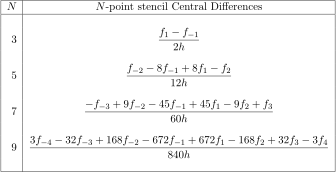
\includegraphics[width=0.9\textwidth]{Figures/centraldifferencecofficients.png}
				\caption{Finite Difference Methods: Central Difference Coefficients \\
				The subscripts $i$ represents  }
				\label{Background:OceanEnvironmentModeling:Figure:centraldifferencecofficients}
			\end{figure}			

			Central differencing is chosen as it is more numerically accurate. The disadvantages of instability and slightly higher time complexity from dynamic cases are not present in the static feature extraction process. Nevertheless, forward differencing is to be used at the boundaries of the dataset where neighboring data is missing on one side.
						
			With two axis, the result is a 2 element gradient vector. It is possible to treat the 2 elements as separate features. However, this would make the modeling problem frame dependent unnecessarily. Therefore, the magnitude of this gradient vector is taken as the slope feature. 
			
			Rugosity is a measure of local height variations in the terrain. By definition, its form is computed as $r = A_{r}/A_{g}$, the real surface area divided by the geometric surface area.
			
			Under cases without perfect grid formation, such as that shown in \cref{Background:OceanEnvironmentModeling:Figure:illustrationBathymetricAgainstLabels}, this feature extraction process becomes only an approximation. As the data set deviates from the form assumed above, it can then become necessary to estimate the features using Gaussian process regression - specifically, the multi-task Gaussian process regression. 
			
		 	On the other hand, under fine-scale bathymetric reconstructions, more sophisticated methods for deriving multi-scale measures of rugosity and slope exist. For example, under bathymetry measurements that are geo-referenced through stereo imagery, rugosity can be calculated through a Delaunay triangulated surface mesh and projecting areas onto the plane of best fit using Principal Component Analysis (PCA) \citep{StefanWilliams:Rugosity}.
							
			\FloatBarrier
				
	\section{Modeling on Test Data Sets}
	
	\section{Comparison: Laplace Approximation and Probabilistic Least Squares}
	
		Compare probability outputs, classification outputs, entropy outputs, etc
	
	\section{Comparison: OVA and AVA methods for multiclass classifiers}
	
	\section{Comparison: Probability fusion methods for multiclass classifiers}
	
%		\subsection{Normalisation Method}
%			
%		\subsection{Mode Keeping}
%			
%		\subsection{Exclusion}
			
	\section{Modeling the Scott Reef Environment}
	
		\subsection{Problems and Solutions to Big Data Analysis}
		
		\subsection{Feature Extraction}
		
		\subsection{Case with 4 Labels}
		
			(With different amounts of sampled points)
			
		\subsection{Case with 17 Labels}
		
	\section{Measuring Mutual Information}
	
		\subsection{Motivation}
			For both modeling purposes and path planning purposes, simply knowing the entropy at each query point is not enough. 
			
		\subsection{Shannon Entropy}
		
		\subsection{Lack of a Closed Form Solution}
		
	\section{A Direct Approach: Monte Carlo Sampling}
		
		\subsection{Development of Methodology}
		
			Provide pseudocode for limited and good way of doing it
			
		\subsection{Binary Classification}
		
		\subsection{Multi-class Classification}
		
	\section{A Faster Approach: Linearised Entropy}
		
		\subsection{Development of Methodology}
		
		\subsection{Binary Classification}
		
			For binary classification, linearisation is performed on the sigmoid, or response, function.
		
			The queried latent vector $\vec{f}$, a finite collection of latent function instances at query points, are distributed as a multivariate Gaussian distribution which can be computed from (equation). 
			
			\begin{equation}
				\vec{f} = [f_{1}, f_{2}, \dots, f_{n_{q}}]^{T} \sim \mathcal{N}(\vec{\mu}, \Sigma)
			\end{equation}
				
			\begin{equation}
				\pi_{i} = \sigma(f_{i}) \qquad \qquad \forall i \in I_{\mathrm{query}} = {1, 2, \dots, n_{q}}
			\end{equation}
			
		\subsection{Multi-class Classification}
		
			For multi-class classification, linearisation is performed on the softmax function for each class.
			
			Provide intuitive reason for the squashing.
			
		

\chapter{Informative Seafloor Exploration}
\lhead{Informative Seafloor Exploration}
\label{InformativeSeafloorExploration}

	The Gaussian process based inference model for benthic habitat mapping devised in Chapter \ref{BenthicHabitatMapping} provides a Bayesian framework for habitat inference and prediction. With such an inference model, this chapter proceeds to develop an informative path planning policy for benthic habitat mapping.
	
	In order to devise an informative path planning policy, it is important to select an appropriate acquisition criterion which measures the desirability of traversing a particular candidate path. Section \ref{Background:RelatedWork} provided an outline of related investigations on various acquisition functions for informative path planning in the benthic habitat mapping context, which motivated the need for a measure of mutual information. Such a measure would allow inference based on the \textit{essential} information contained in any given sub-region of interest. The mutual information criterion can then be employed as the acquisition function for informative path planning, in order to evaluate thus compare the desirability of visiting candidate regions and locations.
	
	Nevertheless, as Gaussian process classifiers lack analytical forms for the predictive joint distribution of target labels, any mutual information measure derived from the predictive joint distribution must rely on numerical estimation techniques. As such, estimating joint prediction information entropy requires a Monte Carlo sampling based approach. Section \ref{InformativeSeafloorExploration:MCJPIE} describes such a mutual information criterion, hereby named Monte Carlo Predictive Information Entropy (MCPIE).
	
	However, a Monte Carlo approach suffers some several drawbacks, such as computational complexity and limited estimation accuracy. Instead, this thesis proposes a new and alternative mutual information measure, Linearised Model Differential Entropy (LMDE), that is more computationally tractable than MCPIE. Section \ref{InformativeSeafloorExploration:LMDE} defines and derives LMDE as an appropriate form of mutual information. Specifically, it regularises between reducing mutual bias and mutual uncertainty through taking advantage of both the latent mean and covariance structure, as well as the non-Gaussian likelihood response. Tractability of the approach is further improved through a linearisation approximation on such an acquisition criterion.
	
	Section \ref{InformativeSeafloorExploration:ComparisonMutualEntropyMeasures} proceeds to demonstrate the two mutual entropy measures through example datasets. Interpretation of the experimental results provides an intuitive understanding of their differences in time complexity, accuracy, and most importantly, their properties.
	
	Section \ref{InformativeSeafloorExploration:RecedingHorizonFormulation} then formulates a receding horizon approach to informative path planning. This provides a simple yet effective framework for a large scale exploration task such as seafloor exploration for benthic habitat mapping. In particular, the receding horizon formulation strikes a balance between exploring in a non-myopic way and doing so with reasonable tractability constraints.
	
	Finally, section \ref{InformativeSeafloorExploration:ScottReef} assesses the performance of various approaches to informative seafloor exploration for benthic habitat mapping. Multiple acquisition criterions are tested under both the receding horizon approach and a myopic greedy approach, which verifies the benefits of linearised model differential entropy under the receding horizon formulation. Under a mapping accuracy criterion, simulations over the Scott Reef dataset demonstrates that LMDE acquisition outperform other criterions, including MCJPIE acquisition.
		
	\section{Monte Carlo Predictive Information Entropy}
	\label{InformativeSeafloorExploration:MCJPIE}
	
		This section introduces the Monte Carlo predictive information entropy (MCPIE) of Gaussian process classifiers. Monte Carlo sampling methods provide a way to estimate the joint predictive entropy through considering the joint distributions of the latent function at the query points.
	
		Monte Carlo sampling, as its name suggests, involve using sampled draws from a particular distribution to estimate a certain quantity that can be characterised by the distribution. In MCPIE case, the distribution to be sampled from is the latent GP process of the GP classifier, whose moments are analytically tractable, and the quantity to be estimated is the predictive information entropy of the query points. A brief description of the method is provided for both binary and multiclass classification.
		
		\subsection{Binary Classification}
		\label{InformativeSeafloorExploration:MCJPIE:Binary}
		
			Suppose a Gaussian process classifier has been trained under Laplace approximation with respect to a training set $\mathcal{D} = \{X, \bvec{y}\} = \{[ \bvec{x}_{1}, \bvec{x}_{2}, \dots, \bvec{x}_{n}]^{T}, [y_{1}, y_{2}, \dots, y_{n}]^{T}\}$ with $n$ training points. It is known that the latent function $f(\bvec{x})$ is distributed as a GP with a particular predictive mean $m(\bvec{x})$ and covariance $k(\bvec{x}, \bvec{x}')$ once conditioned on the training data \eqref{Equation:PredictiveLatentBinaryGP}. Note that again this section will omit explicitly notating the training data and query data that was conditioned upon. \begin{equation}
				f(\bvec{x}) \sim \mathcal{GP}(m(\bvec{x}), k(\bvec{x}, \bvec{x}'))
			\label{Equation:PredictiveLatentBinaryGP}
			\end{equation}
			
			Let $X^{\star} = [ \bvec{x}^{\star}_{1}, \bvec{x}^{\star}_{2}, \dots, \bvec{x}^{\star}_{n^{\star}}]^{T}$ denote the collection of $n^{\star}$ query points for which inference is to be performed upon. Denote $\bvec{f}^{\star}$ the vector of latent function values $f^{\star}_{i} = f(\bvec{x}^{\star}_{i})$ at each query point. By definition of a GP, $\bvec{f}^{\star}$ is multivariate Gaussian distributed with corresponding means $\mu^{\star}_{i} = m(\bvec{x}^{\star}_{i})$ and covariances $\Sigma^{\star}_{ij} = k(\bvec{x}^{\star}_{i}, \bvec{x}^{\star}_{j})$ \eqref{Equation:BinaryPredictiveGaussianDistribution}. \begin{equation}
				\bvec{f}^{\star} = [f^{\star}_{1}, f^{\star}_{2}, \dots, f^{\star}_{n^{\star}}]^{T} \sim \mathcal{N}(\vec{\upmu}^{\star}, \Sigma^{\star})
			\label{Equation:BinaryPredictiveGaussianDistribution}
			\end{equation}
				
			The binary prediction probability $\vec{\uppi^{\star}}$ at the query points is obtained through passing the queried latent function random vector $\bvec{f}^{\star}$ through a response function in a component wise fashion \eqref{Equation:PredictiveResponse}. \begin{equation}
				\vec{\uppi}^{\star} = \vec{\upsigma}(\bvec{f}^{\star})\mathrm{ \quad i.e. \;\;}\pi^{\star}_{i} = \sigma(f^{\star}_{i}) \quad \forall i \in I_{n^{\star}}
			\label{Equation:PredictiveResponse}
			\end{equation}
			
			As a straightforward transformation of the latent vector, the predictive probability vector $\vec{\uppi^{\star}}$ is thus a random vector itself. The usual procedure is then to treat the expected prediction probabilities $\mathbb{E}[\vec{\uppi^{\star}}]$ as the posterior class probabilities for further inference. However, this discards any information regarding the joint behaviour of an arbitrary collection of query points. As a result, a measure of mutual information shared amongst the query points cannot be obtained.
			
			As such, one straightforward approach to address this problem is to perform Monte Carlo estimation of the posterior joint distribution for class predictions via jointly sampling latent vectors from the GP latent, whose distribution is completely characterised through \eqref{Equation:PredictiveLatentBinaryGP} and definition \ref{Definition:GaussianRandomField}. For each jointly sampled vector, the components with positive latent values are assigned class label 1, and -1 otherwise. That is, for a particular sample ${^{s}}\bvec{f}^{\star}$ drawn from $\bvec{f}^{\star} \sim \mathcal{N}(\vec{\upmu}^{\star}, \Sigma^{\star})$ \eqref{Equation:BinaryPredictiveGaussianDistribution}, $s \in I_{n_{S}}$ where $n_{S}$ is the number of samples, the corresponding class assignments are computed through \eqref{Equation:MonteCarloSamplingBinaryClassifier}. Here, the left superscript $s$ indexes the sampled value or vector. As before, without the left superscript $s$, $\bvec{f}^{\star}$ is a random vector, while ${^{s}}\bvec{f}^{\star}$ is a particular realised, fixed vector. \begin{equation}
				{^{s}}\bvec{y}^{\star} = \bvec{\mathds{H}}({^{s}}\bvec{f}^{\star}) := \{\mathbb{H}({^{s}}f^{\star}_{i})\}_{i \in I_{n^{\star}}} \quad \forall s \in I_{n_{s}} \quad \mathrm{where} \quad \mathbb{H}(z) := \mathds{1}_{z > 0} - \mathds{1}_{z \leq 0}
			\label{Equation:MonteCarloSamplingBinaryClassifier}
			\end{equation}
			
			where $\mathbb{H}(z)$ is the modified Heaviside function which is 1 is $z$ is positive and -1 otherwise, so that ${^{s}}\bvec{y}^{\star} \in \{-1, 1\}^{n_{S}}$. Note that the sampled labels can be determined completely from the sampled latent function as, once sampled, the latent function is no longer a random function. Hence, any positive (negative) latent values will map to prediction probabilities of more (less) than 0.5 under any likelihood response.
			
			Further, define $I_{U} \subseteq I_{n_{S}}$, $n_{U} := \Vert I_{U} \Vert$, as the indices corresponding to the subset with the maximum amount of unique samples \eqref{Equation:UniqueIndexSet}.
			
			\begin{equation}
				I_{U} := \argmax_{\{I \subseteq I_{n_{S}} | {^{s}}\bvec{y}^{\star} \neq {^{t}}\bvec{y}^{\star}, \forall s, t \in I\}} \Vert I \Vert 
			\label{Equation:UniqueIndexSet}
			\end{equation}			
			
			where $\Vert I \Vert$  stands for the cardinality of $I$. An \textit{estimated} probability vector $\tilde{\bvec{p}}$ can then be formed \eqref{Equation:EstimatedProbability}.

			\begin{equation}
				\begin{aligned}
					\tilde{\bvec{p}}^{\star} &:= \bigg\{ \frac{1}{n_{S}}\mathbb{F}_{I_{n_{S}}}({^{s}}\bvec{y}^{\star}) \bigg\}_{s \in I_{U}} \\
					\mathbb{F}_{I_{n_{S}}}({^{s}}\bvec{y}^{\star}) &:= \sum_{t \in I_{n_{S}}} \mathds{1}_{{^{s}}\bvec{y}^{\star} = {^{t}}\bvec{y}^{\star}}
				\end{aligned}
			\label{Equation:EstimatedProbability}
			\end{equation}
			
			where $\mathbb{F}_{I_{n_{S}}}({^{s}}\bvec{y}^{\star})$ is the frequency of appearance of the vector ${^{s}}\bvec{y}^{\star}$ amongst all the sampled vectors $\{ {^{s}}\bvec{y}^{\star} \}_{s \in I_{n_{S}}}$. Note that each \textit{unique} sample is assigned a probability such that the vector $\tilde{\bvec{p}}^{\star}$ has exactly $n_{U}$ non-zero entries indexed by $I_{U}$, which is generally smaller than the total number of possible samples. This inherently means that possible samples that were not drawn or \textit{realised} are estimated with probability zero. In this way, since more samples would likely realise those unlikely possibilities and thus raising the corresponding probability to a nonzero value, estimation accuracy will benefit from higher numbers of samples $n_{S}$.
			
			Finally,  for $n_{C} = 2$ classes, the Monte Carlo predictive information entropy, as an instance of Shannon entropy \eqref{Equation:DiscreteEntropy}, can be computed from the estimated probabilities that represent the joint distribution \eqref{Equation:MCPIE}. As usual, only non-zero entries of $\tilde{\bvec{p}}$ need to be considered. 
			
			\begin{equation}
				H_{\mathrm{MCPIE}} \stackrel{\text{abbrev.}}{:=} H_{\mathrm{MCPIE}}[X^{\star} | X, \bvec{y}] := - \sum_{i \in I_{n_{U}}} \tilde{p}^{\star}_{i} \log(\tilde{p}^{\star}_{i})
			\label{Equation:MCPIE}
			\end{equation}		
			
		\subsection{Multiclass Classification}
		\label{InformativeSeafloorExploration:MCJPIE:Multiclass}
		
			The derivation in the multiclass case is similar to the binary case. Specifically, since ${^{s}}\bvec{y}^{l} \in \{1, 2, \dots, n_{C}\}^{n_{s}}$ it suffices to replace the sampling step \eqref{Equation:MonteCarloSamplingBinaryClassifier} with \eqref{Equation:MonteCarloSamplingMulticlassClassifier}.
			
			The following sampling method assumes that the GP classifier has been trained under a OVA scheme (see section \ref{BenthicHabitatMapping:Classification:MulticlassClassification:OVA}). Analogous to \eqref{Equation:PredictiveLatentBinaryGP}, for $c$ classes, there are $n_{C}$ latent functions $\{f^{1}(x), f^{2}(x), \dots, f^{n_{C}}(x)\}$ corresponding to each class \eqref{Equation:PredictiveLatentMulticlassGP}. \begin{equation}
				f^{c}(\bvec{x}) \sim \mathcal{GP}(m^{c}(\bvec{x}), k^{c}(\bvec{x}, \bvec{x}')) \qquad \forall c \in I_{n_{C}}
			\label{Equation:PredictiveLatentMulticlassGP}
			\end{equation}
						
			Here the superscript $c$ is used to index the classes. The latent vector $\bvec{f}_{i} := \{f^{c}_{i}\}_{c \in I_{n_{C}}}$ represents the collection of $n_{C}$ latent values across classes at the query point $i \in I_{n^{\star}}$, and is distinct from $\bvec{f}^{c} := \{f^{c}_{i}\}_{i \in I_{n^{\star}}}$ which represents the collection of $n^{\star}$ latent values across query points for class $c \in I_{n_{C}}$.
			
			Again, by definition of a GP, each ${\bvec{f}^{c}}^{\star}$ is multivariate Gaussian distributed with corresponding means ${\mu^{c}}^{\star}_{i} = m^{c}(\bvec{x}^{\star}_{i})$ and covariances ${\Sigma^{c}}^{\star}_{ij} = k^{c}(\bvec{x}^{\star}_{i}, \bvec{x}^{\star}_{j})$ \eqref{Equation:MulticlassPredictiveGaussianDistribution}. \begin{equation}
				{\bvec{f}^{c}}^{\star} = [{f^{c}}^{\star}_{1}, {f^{c}}^{\star}_{2}, \dots, {f^{c}}^{\star}_{n^{\star}}]^{T} \sim \mathcal{N}({\vec{\upmu}^{c}}^{\star}, {\Sigma^{c}}^{\star})
			\label{Equation:MulticlassPredictiveGaussianDistribution}
			\end{equation}
			
			For each class $c$, a sample ${^{s}}{\bvec{f}^{c}}^{\star}$ is drawn from ${\bvec{f}^{c}}^{\star} \sim \mathcal{N}({\vec{\upmu}^{c}}^{\star}, {\Sigma^{c}}^{\star})$, where $s \in I_{n_{S}}$. The corresponding sampled target labels are then found by \eqref{Equation:MonteCarloSamplingMulticlassClassifier}. \begin{equation}
				\begin{aligned}
					{^{s}}\bvec{y}^{\star} = \bvec{\mathds{M}}_{n_{C}}({^{s}}{\bvec{f}^{1}}^{\star}, {^{s}}{\bvec{f}^{2}}^{\star}, \dots, {^{s}}{\bvec{f}^{n_{C}}}^{\star}) &:= \{\mathbb{M}_{n_{C}}({^{s}}{f^{1}}^{\star}_{i}, {^{s}}{f^{2}}^{\star}_{i}, \dots, {^{s}}{f^{n_{C}}}^{\star}_{i})\}_{i \in I_{n^{\star}}} \quad \forall s \in I_{n_{s}} \\
					\mathrm{where} \qquad \mathbb{M}_{n_{C}}(z_{1}, z_{2}, \dots, z_{n_{C}}) &:= \argmax_{c \in I_{n_{C}}} z_{c}
				\end{aligned}
			\label{Equation:MonteCarloSamplingMulticlassClassifier}
			\end{equation}
			
			That is, for each sample $s \in I_{n_{S}}$ and at each query point $i \in I_{n^{\star}}$, ${^{s}}y^{\star}_{i}$ is assigned the class label from $\{1, 2, \dots, n_{C}\}$ that has the maximal latent value. With the samples $\{{^{s}}\bvec{y}^{\star}\}_{s \in I_{n_{s}}}$, the estimated probability can be computed from \eqref{Equation:EstimatedProbability}, so that the Monte Carlo predictive information entropy for $n_{C} > 2$ classes can also be computed from \eqref{Equation:MCPIE}.
			
	\section{Linearised Model Differential Entropy}
	\label{InformativeSeafloorExploration:LMDE}
	
		This section introduces the linearised model differential entropy (LMDE) of Gaussian process classifiers. This method attempts to address the need for a measure of mutual entropy that is more computationally viable compared than Monte Carlo methods. Through investigating the structure of the GP classification inference model in both the binary and multiclass classification setting, a simple derivation for LMDE is provided.
		
		\subsection{Binary Classification}
		\label{InformativeSeafloorExploration:LMDE:Binary}
		
			For binary classification, linearisation is performed on the likelihood response.
					
			The beginning of this derivation is the same as section \ref{InformativeSeafloorExploration:MCJPIE:Binary} up to \eqref{Equation:PredictiveResponse}. At this stage, instead of proceeding with Monte Carlo sampling, it is proposed to use the joint distribution of the predictive probabilities $\vec{\uppi^{\star}}$ itself as a basis of constructing a measure of mutual information. Unlike traditional approaches where inference depends only on the expectance $\mathbb{E}[\vec{\uppi^{\star}}]$ such that structural information from the latent GP is compromised, it is aimed to utilise also the covariance $\mathbb{V}[\vec{\uppi^{\star}}]$, which contains information regarding both the latent GP and the response likelihood.
		
			\begin{figure}[!htbp]
				\centering
					\includegraphics[width = 0.6\linewidth]{Figures/linearisation.eps}
				\caption{Linearisation accuracy for a probit response: Green shade represents the latent variance while blue shade represents the predictive variance. Gold lines show local linearisation about latent expectance.}
				\label{Figure:Linearisation}
			\end{figure}
				
			As the predictive probabilities are nonlinear transformations of the Gaussian distributed latent vector, they are no longer Gaussian distributed. In order to retain analytical tractability, the proposed approach is to linearise the response function about the latent expectance $\bar{f}^{\star}_{i} := \mathbb{E}[f^{\star}_{i}]$. Figure \ref{Figure:Linearisation} illustrates the linearisation accuracy for a probit response. Observe that points with latent expectance far away from zero translate to near zero predictive variance even under high latent variance. Linearisation is thus very accurate for those points. For points with latent expectances near zero, we require the latent variances to be sufficiently small for linearisation to be accurate.
			
			The linearised can thus be derived, which also serves to construct the definition of linearised differential entropy. With first order Taylor expansion, the response is linearised the latent mean $\bar{f}^{\star}_{i} = \mathbb{E}[f^{\star}_{i}]$ \eqref{Equation:LinearisingSigmoid}. \begin{equation}
				\sigma(f^{\star}_{i}) \approx \sigma_{L}(f^{\star}_{i}) := \sigma(\bar{f}^{\star}_{i}) + \sigma'(\bar{f}^{\star}_{i}) (f^{\star}_{i} - \bar{f}^{\star}_{i})
			\label{Equation:LinearisingSigmoid}
			\end{equation}
			
			The prediction probabilities are now approximated as a linear transformation $\sigma_{L}(f)$ of the latent vector, so that it is also multivariate Gaussian distributed with expectance and covariance available in analytical form \eqref{Equation:MomentsLinearisedSigmoid}. \begin{align*}
			\numberthis \label{Equation:MomentsLinearisedSigmoid}
					\vec{\upsigma}_{L}(\bvec{f}^{\star}) & \sim \mathcal{N}(\vec{\upmu}^{\star}_{L}, \Sigma^{\star}_{L}) \\
					({\mu^{\star}_{L}})_{i} & = \mathbb{E}[\sigma_{L}(f^{\star}_{i})] = \sigma(\bar{f}^{\star}_{i}) \\
					({\Sigma^{\star}_{L}})_{ij} & = \mathbb{C}\mathrm{ov}[\sigma_{L}(f^{\star}_{i}), \sigma_{L}(f^{\star}_{j})] = \sigma'(\bar{f}^{\star}_{i}) \sigma'(\bar{f}^{\star}_{j}) \mathbb{C}\mathrm{ov}[f^{\star}_{i}, f^{\star}_{j}]
			\end{align*}
			
			Finally, the linearised model differential entropy $H_{\mathrm{LMDE}}$ at the query points $X^{\star}$ is defined to be the differential entropy corresponding to the random vector $\vec{\upsigma}_{L}(\bvec{f}^{\star})$. Since $\vec{\upsigma}_{L}(\bvec{f}^{\star})$ is multivariate Gaussian distributed, $H_{\mathrm{LMDE}}$ exhibits a closed form \eqref{Equation:BinaryLinearisedEntropy}. \begin{equation}
				H^{\mathrm{binary}}_{\mathrm{LMDE}} \stackrel{\text{abbrev.}}{:=} H^{\mathrm{binary}}_{\mathrm{LMDE}}[X^{\star} | X, \bvec{y}] := \frac{1}{2} \log\Big((2 \pi e)^{n^{\star}} \det(\Sigma^{\star}_{L})\Big)
			\label{Equation:BinaryLinearisedEntropy}
			\end{equation}			
						
		\subsection{Multiclass Classification}
		\label{InformativeSeafloorExploration:LMDE:Multiclass}
		
			For multiclass classification, linearisation is performed on the softmax function $\sigma^{c}$ which returns the corresponding predictive class probability $\vec{\uppi}^{c}$ for class $c \in I_{n_{C}} := \{1, 2, \dots, n_{C}\}$ \eqref{Equation:Softmax} \citep{GaussianProcessForMachineLearning}. \begin{equation}
				{\pi^{c}_{i}}^{\star} = \sigma^{c}({\bvec{f}_{i}}^{\star}) := \frac{\exp({f^{c}_{i}}^{\star})}{\sum_{m = 1}^{n_{C}} \exp({f^{m}_{i}}^{\star})} \qquad c \in I_{n_{C}}
			\label{Equation:Softmax}
			\end{equation}
			
			Again, OVA classifiers are employed, where each class is trained against all other classes independently with a binary classifier. For $c$ classes, $c$ binary classifiers are trained independently and also performs inference independently. The normalisation is then inherently captured in the softmax \eqref{Equation:Softmax}. This approach avoids the Monte Carlo sampling step in the inference stage of a typical GP multiclass classifier under Laplace Approximation \citep{GaussianProcessForMachineLearning}, and is thus faster in computational time. Note that this Monte Carlo sampling step avoided is separate to the one used in MCJIE. In essence, using OVA classifiers skip one Monte Carlo step, and using LMDE skips another Monte Carlo step through avoiding using MCPIE. Furthermore, because each classifier is trained independently, both the learning stage and the inference stage can be performed in parallel, further speeding up the process in a way that was not available under the original scheme. This is important later in under a receding horizon formulation, where the inference stage is included in the objective function of an optimiser such that repeated evaluations would benefit dramatically from shorter inference time.
			
			Similar to the binary case, to linearise it is imperative to examine the gradient of each of the $c$ softmax functions \eqref{Equation:SoftmaxGradient}. For notational simplicity, the query stars ($^{\star}$) are omitted in this derivation except for $n^{\star}$.
			
			\begin{equation}
				\frac{\partial \sigma^{c}}{\partial f^{k}_{i}}(\bvec{f}_{i}) =
				\begin{cases} 
					- \frac{\exp(f^{c}_{i}) \exp(f^{k}_{i})}{\sum_{m = 1}^{n_{C}} \exp({f^{c}_{i}})} & \text{for } k \neq c  \\
					- \frac{\exp(f^{c}_{i})^{2}}{\big(\sum_{m = 1}^{n_{C}} \exp({f^{c}_{i}})\big)^{2}} + \frac{\exp(f^{c}_{i})}{\sum_{m = 1}^{n_{C}} \exp({f^{c}_{i}})}& \text{for } k = c
				\end{cases}
			\label{Equation:SoftmaxGradient}
			\end{equation}			
		
			The numerators are explicitly left in the form of products of exponentiation instead of exponentiation of sums to reflect ways to cache quantities during computation. 
			
			Hence, for each class $c$ at query point $i$ a softmax gradient vector is computed \eqref{Equation:SoftmaxGradientVector}.
			
			\begin{equation}
				\frac{\partial \sigma^{c}}{\partial \bvec{f}_{i}}(\bvec{f}_{i}) := \begin{bmatrix} \frac{\partial \sigma^{c}}{\partial f^{1}_{i}}(\bvec{f}_{i}) & \frac{\partial \sigma^{c}}{\partial f^{2}_{i}}(\bvec{f}_{i}) & \dots & \frac{\partial \sigma^{c}}{\partial f^{n_{C}}_{i}}(\bvec{f}_{i}) \end{bmatrix}^{T}
			\label{Equation:SoftmaxGradientVector}
			\end{equation}
			
			The linearisation is again performed on the mean latent predictions $\bar{\bvec{f}}_{i} = \mathbb{E}[\bvec{f}_{i}]$ so that each softmax $\sigma^{c}(\bvec{f}_{i})$ can be approximated with the linearised softmax $\sigma^{c}_{L}(\bvec{f}_{i})$ \eqref{Equation:LinearisedSoftmax} in an analogous form as \eqref{Equation:LinearisingSigmoid}.
			
			\begin{equation}
				\begin{aligned}
					\sigma^{c}(\bvec{f}_{i}) \approx \sigma^{c}_{L}(\bvec{f}_{i}) & := \sigma^{c}(\bar{\bvec{f}}_{i}) + \left. \frac{\partial \sigma^{c}}{\partial \bvec{f}_{i}} \right|^{T}_{\bvec{f}_{i} = \bar{\bvec{f}}_{i}} (\bvec{f}_{i} - \bar{\bvec{f}}_{i}) \\
					& = \bvec{a}^{c}_{i} + (\bvec{g}^{c}_{i})^{T} (\bvec{f}_{i} - \bar{\bvec{f}}_{i})
				\end{aligned}
			\label{Equation:LinearisedSoftmax}
			\end{equation}
			
			where we have notated the constants $\bvec{a}^{c}_{i} := \sigma^{c}(\bar{\bvec{f}}_{i})$ and $\bvec{g}^{c}_{i} := \frac{\partial \sigma^{c}}{\partial \bvec{f}_{i}}(\bar{\bvec{f}}_{i})$.
			
			To determine the distribution of the vector of softmax values across query points, first define the following \eqref{Equation:Definitions}.
			
			\begin{equation}
				\begin{aligned}
					F &:= \{f^{c}_{i}\}_{c \in I_{n_{C}}, i \in I_{n^{\star}}} \in \mathbb{R}^{n_{C} \times n^{\star}} \\
					\vec{\upsigma}^{c}_{L}(F) &:= \begin{bmatrix} \sigma^{c}_{L}(\bvec{f}_{1}) & \sigma^{c}_{L}(\bvec{f}_{2}) & \dots & \sigma^{c}_{L}(\bvec{f}_{n^{\star}}) \end{bmatrix}^{T} \qquad \forall c \in I_{n_{C}}
				\end{aligned}
			\label{Equation:Definitions}
			\end{equation}
						
			The covariance of the linearised softmax of a particular class $c$ between two query points $i$ and $j$ can now be computed, as well as the expectance at a particular query point $i$ \eqref{Equation:MomentsLinearisedSoftmax}.
			
			\begin{align*}
			\numberthis \label{Equation:MomentsLinearisedSoftmax}
					\vec{\upsigma}^{c}_{L}(F) & \sim \mathcal{N}(\vec{\upmu}^{c}_{L}, \Sigma^{c}_{L}) \\
					(\mu^{c}_{L})_{i} & = \mathbb{E}[\sigma^{c}_{L}(\bvec{f}_{i})] =  \sigma^{c}(\bar{\bvec{f}}_{i}) \\
					(\Sigma^{c}_{L})_{ij} & = \mathbb{C}\mathrm{ov}[\sigma^{c}_{L}(\bvec{f}_{i}), \sigma^{c}_{L}(\bvec{f}_{i})] \\
					& = \mathbb{C}\mathrm{ov}[(\bvec{g}^{c}_{i})^{T} \bvec{f}_{i}, (\bvec{g}^{c}_{j})^{T} \bvec{f}_{j}] \\
					& = \sum_{m = 1}^{n_{C}} (g^{c}_{i})^{m} (g^{c}_{j})^{m} \mathbb{C}\mathrm{ov}[f^{m}_{i}, f^{m}_{j}]
			\end{align*}
						
			where $(g^{c}_{i})^{m}$ denotes the $m^{\text{th}}$ element of $\bvec{g}^{c}_{i}$. The last equality arises as a result of employing OVA multiclass classification, where latent values of classes $c$ and $m$, $c \neq m$, are conditionally independent given training observations.
			
			Finally, the linearised entropy of the OVA multiclass Gaussian process classifier is defined as follows \eqref{Equation:MulticlassLinearisedEntropy}. \begin{equation}
				H^{\mathrm{multiclass}}_{\mathrm{LMDE}} \stackrel{\text{abbrev.}}{:=} H^{\mathrm{multiclass}}_{\mathrm{LMDE}}[X^{\star} | X, \bvec{y}] := \frac{1}{2} \log\Bigg((2 \pi e)^{n^{\star}} \det\bigg(\sum_{c = 1}^{n_{C}} \Sigma^{c}_{L}\bigg)\Bigg)
			\label{Equation:MulticlassLinearisedEntropy}
			\end{equation}
		
	\section{Comparison of Mutual Entropy Measures}
	\label{InformativeSeafloorExploration:ComparisonMutualEntropyMeasures}
	
		Both Monte Carlo prediction information entropy and linearised model differential entropy are suitable measures of mutual entropy that can be used as an acquisition criterion for informative path planning. This section provides a simple comparison between the two entropy measures with example datasets, which would further assist in the interpretation of model differential entropy. The main takeaway is that MCPIE and LMDE are complementary measures of entropy which together captures uncertainty in prediction and uncertainty in the model respectively.
	
		\subsection{Estimation Accuracy under Monte Carlo Sampling}
		
			It is helpful to visualise the practical numbers of samples required for reasonable estimation accuracy for MCPIE. Figure \ref{Figure:mcpie_lmde_comparison_binary} shows a simple case for a binary classification scenario, while Figure \ref{Figure:mcpie_lmde_comparison_multiclass} shows a case for a multiclass classification scenario with 4 classes. 
			
			\begin{figure}[!htbp]
				\centering
					\includegraphics[width = \linewidth]{Figures/mcpie_lmde_comparison_binary/mcpie_lmde_comparison.eps}
				\caption{GP binary classifier example}
				\label{Figure:mcpie_lmde_comparison_binary}
			\end{figure}			
						
			In both cases, the training data are evenly distributed in the feature space with features $x_{1}$ and $x_{2}$. In both Figure \ref{Figure:mcpie_lmde_comparison_binary} and \ref{Figure:mcpie_lmde_comparison_multiclass}, the MCPIEs are estimated with 2500 samples \textit{at each query point}. Note that only the marginalised entropies can visualised, as it is difficult to visualise multiple regional entropies. However, this is sufficient to provide an intuition for the accuracy of the method.
			
			\begin{figure}[!htbp]
				\centering
					\includegraphics[width = \linewidth]{Figures/mcpie_lmde_comparison_multiclass/mcpie_lmde_comparison.eps}
				\caption{GP multiclass classifier example}
				\label{Figure:mcpie_lmde_comparison_multiclass}
			\end{figure}
			
			Since only the marginalised entropies are visualised, there exists analytical forms for prediction information entropy by computing the Shannon entropy over the expected prediction probabilities at each query point. For a multiclass case under the OVA formulation, the probabilities are fused using the \textit{exclusion} method (see section  \ref{BenthicHabitatMapping:Classification:ProbabilityFusion:Exclusion}). Subplots (2, 1) and (2, 2) of Figures \ref{Figure:mcpie_lmde_comparison_binary} and \ref{Figure:mcpie_lmde_comparison_multiclass} show the analytically computed PIE and Monte Carlo estimated PIE (MCPIE) respectively. Both cases show that with 2500 samples, the estimation is fairly accurate.
			
			\begin{figure}[!htbp]
				\centering
					\includegraphics[width = \linewidth]{Figures/mcpie_lmde_comparison_binary/mcpie_accuracy.eps}
				\caption{Accuracy improvement of MCPIE for a binary case}
				\label{Figure:mcpie_accuracy_binary}
			\end{figure}
				
			Figures \ref{Figure:mcpie_accuracy_binary} and \ref{Figure:mcpie_accuracy_multiclass} visualises the accuracy improvement as more samples are used for entropy estimation in the corresponding binary and multiclass case respectively. With low numbers of samples, the estimation is noisy and inaccurate, and generally converges to a reasonable accuracy after 1000 samples. Notice however that even with low numbers of samples, the entropies are mostly in the correct range already.
			
			\begin{figure}[!htbp]
				\centering
					\includegraphics[width = \linewidth]{Figures/mcpie_lmde_comparison_multiclass/mcpie_accuracy.eps}
				\caption{Accuracy improvement of MCPIE for a multiclass case}
				\label{Figure:mcpie_accuracy_multiclass}
			\end{figure}
			
		\subsection{Interpretation of Model Differential Entropy}
		\label{InformativeSeafloorExploration:LMDE:Interpretation}
		
			It is worthwhile to remember that model differential entropy and its linearisation is not an approximation to the usual prediction information entropy - the former is a differential entropy on a multivariate Gaussian distribution and the latter is an information entropy on the distribution of discrete class predictions combinations, which is a multivariate multinomial distribution. They have different interpretations and both can have advantageous properties under different scenarios. It is proposed that using linearised model differential entropy as an alternative acquisition function for informative path planning can be more beneficial under specific exploration purposes.
			
			Specifically, while the prediction information entropy (PIE) represents the confidence in the model, the model differential entropy (MDE) represents the the separability of classes in the feature space. In fact, MDE quantifies the ambiguity of the predictive probabilities. In particular, it is possible for GP multiclass classifiers to conclude low predictive variance even under uncertain predictive probabilities. In this case, the MDE would be high while the PIE would be low at such locations, indicating that the model is confident about its inability to separate classes \citep{AsherBender}. Similar to the bias-variance trade-off, such a situation indicate high bias, and is distinct from a model that is unconfident about its ability to separate classes, which would correspond to high variance. In fact, as the entropy of the prediction probabilities, model differential entropy is so named as it measures the uncertainty in the model itself. While an uncertainty in the model propagates into uncertainty in the prediction, it also propagates into bias in the prediction as an inaccurate model is unlikely to predict the correct class labels on average. This demonstrates that PIE and MDE are two complementary measures of entropy that can assist each other in identifying both places of high bias and high variance.
			
			In this way, using MDE as the acquisition function means that the vehicle would prioritise on both getting the both the model and predictions as correct as possible, instead of only focusing on predictions as in the PIE case.
			
		\subsection{Advantage of Model Differential Entropy}
		
			Here the examples from Figures \ref{Figure:mcpie_lmde_comparison_binary} and \ref{Figure:mcpie_lmde_comparison_multiclass} are discussed further in detail.
			
			With abundant and evenly distributed training data, the classifiers achieves a misclassification rate of only 2.2\% and 8.6\% respectively. The classifiers are trained with an axis aligned Gaussian kernel with a probit response under Laplace approximation. 
			
			Intuitively, under abundant data, it is desired that the classifier would only indicate high entropies at decision boundaries. In Figure \ref{Figure:mcpie_lmde_comparison_binary}, the prediction information entropy is indeed near its maximum at the predicted decision boundaries. As an artefact of the Laplace approximation, however, it is also quite high around the edges where the classifier has learned a slightly lower signal to noise ratio. In this example, there are no training points around the edges shown. As a result, the GP classifier learns a slightly lower signal to noise ratio in the latent function, and bounces back to its latent GP prior for which it remains uncertain regarding class label assignments. The prediction information entropy reflects this change more rapidly, so that it is high both at the decision boundaries and wherever observations are lacking. If the acquisition function for informative exploration is a function of the prediction information entropy, the vehicle would be suggested to explore both places with lacking observations and the decision boundaries. 
	
			This leads to the classic exploration-exploitation dilemma most machine learning algorithms face. It is possible that there exists decision boundaries yet to be detected at regions of lower relative data density. Is it worth it for the vehicle to explore and discover such regions, or exploit the currently known boundaries and map it better? In most exploration applications, the priority is to map the region of interest as accurately and fast as possible in order to reduce time and cost. While it is possible that there exists undiscovered decision boundaries at regions of lower relative data density, it is undesirable under cost constraints that this possibility is weighed heavily by the vehicle even under abundant data.
					
			On the other hand, linearised model differential entropy focuses on the decision boundary as it is constructed to be only high when the latent function is near zero (figure \ref{Figure:Linearisation}). Figure \ref{Figure:mcpie_lmde_comparison_binary} shows that that LMDE emphasizes on where the latent expectance is close to zero, and filters out the rest. If LMDE is used as the acquisition function, the vehicle would focus on the decision boundaries within the feature space, so that the vehicle would focus strictly on the mapping the predicted decision boundaries better. Notice that regions far away from observations in the feature space are also assigned with high linearised differential entropy, as the latent function bounces back to its prior, so that the vehicle would explore those parts of the feature space if necessary.
			
			Figure \ref{Figure:mcpie_lmde_comparison_multiclass} shows a similar scenario with a multi-class scenario with 4 labels. The same behaviour as the binary case is observed, where the LMDE approach pushes down the entropy level of all regions except the predicted decision boundaries.

			Furthermore, in the case of a feature space that does not contain the spatial coordinates for which path planning in based on, the MCPIE method may spent a lot of time in a single region where it is locally rich in span of a subspace of the feature space. However, this is suboptimal as this means it is giving up on trying to go for other regions that may have an even richer span of the feature space. The linearised model differential entropy method focuses its efforts (prioritises) the decision boundaries in the feature space at the expense of overlooking regions with less observations. This leads to smoother paths as it will look at all elements of the feature space. As long as one of the features is spatially correlated (depth in the benthic habitat mapping case), this will lead to smoother paths.
	
% 62500 QUERIES [MARGINALISED]
	
% BINARY 1: INFO:root:{'time_mcpie_high': 18.39458680280154, 'time_mcpie_med': 2.383764856014338, 'time_lmde': 0.009482532012810907, 'time_mcpie_low': 1.3273178461480555, 'time_pie': 0.0020675683150006563}

% MULTICLASS 1: INFO:root:{'time_mcpie_low': 2.2666649940613013, 'time_pie': 0.0048935111084738026, 'time_mcpie_med': 14.068846717692534, 'time_lmde': 0.18608571000102003, 'time_mcpie_high': 161.86858168576953}

% 30 QUERIES [MUTUAL]

% BINARY 2: INFO:root:{'time_mcpie_high': 0.008627792656996647, 'time_mcpie_low': 0.0014215244923594383, 'time_lmde': 0.0005034922289421928, 'time_pie': 3.877403348617747e-05, 'time_mcpie_med': 0.0022112603214488047}

% MULTICLASS 2: INFO:root:{'time_lmde': 0.00633157158570441, 'time_mcpie_med': 0.016457866595658288, 'time_mcpie_high': 0.7391853233440777, 'time_mcpie_low': 0.0015897353729243946, 'time_pie': 3.250176336422328e-05}

% 300 QUERIES [MUTUAL]

% BINARY 3: INFO:root:{'time_mcpie_high': 4.936638667632977, 'time_pie': 5.245898648098546e-05, 'time_lmde': 0.0069382711684848886, 'time_mcpie_med': 0.09106880053097655, 'time_mcpie_low': 0.008598141925508784}

% MULTICLASS 3: INFO:root:{'time_mcpie_med': 0.12034433622561025, 'time_lmde': 0.388328217631809, 'time_mcpie_low': 0.02316748500784982, 'time_mcpie_high': 5.203110931939598, 'time_pie': 5.245898648098546e-05}

% 1000 QUERIES [MUTUAL]

% BINARY 4: INFO:root:{'time_mcpie_high': 17.58592924537178, 'time_pie': 9.636487733999388e-05, 'time_mcpie_low': 0.048404819156196766, 'time_lmde': 0.05436689701103603, 'time_mcpie_med': 0.2604223746700658}

% MULTICLASS 4: INFO:root:{'time_mcpie_high': 18.22034028776035, 'time_lmde': 3.460213565095618, 'time_pie': 0.00012886664070421716, 'time_mcpie_med': 0.5077237304497615, 'time_mcpie_low': 0.1775907754293513}

		\begin{table}[h]
			\begin{center}
				\begin{tabular}{ l c c c c }
					\hline
					\hline
					Test Cases & MCPIE (low) & MCPIE (medium) & MCPIE (high) & LMDE \\
					\hline
					\hline
					Binary 1 & 1.3273 & 2.3837 & 18.3945 & 0.0094 \\
					Multiclass 1 & 2.2666 & 14.0688 & 161.8685 & 0.1860 \\
					Binary 2 & 0.0014 & 0.0022 & 0.0086 & 0.0005 \\
					Multiclass 2 & 0.0015 & 0.01645 & 0.7391 & 0.0063 \\
					Binary 3 & 0.0085 & 0.0910 & 4.9366 & 0.0069 \\
					Multiclass 3 & 0.0231 & 0.1203 & 5.2031 & 0.3883 \\
					Binary 4 & 0.0484 & 0.2604 & 17.5859 & 0.0543 \\
					Multiclass 4 & 0.1775 & 0.5077 & 18.2203 & 3.4602 \\
					\hline
					\hline
				\end{tabular}
			\end{center}
	  	\caption{Average Time Complexity Performance in Seconds \\ Low, medium, and high refers to the number of samples used [25, 250, 2500] \\ Case 1: Computing marginalised entropy over 62500 queries \\ Cases [2, 3, 4]: Computing mutual entropy over [30, 300, 1000] queries}
	  	\label{Table:TimeComplexity}			
	  	\end{table}	
	  	
		Finally, in terms of time complexity, Table \ref{Table:TimeComplexity} shows experimental results for the computational time required for different cases, averaged over 10 trials for each computation. Specifically, case 1 refers to the computations that generated the LDME in Figures \ref{Figure:mcpie_lmde_comparison_binary} and \ref{Figure:mcpie_lmde_comparison_multiclass}, and the MCPIEs with various numbers of samples in Figures \ref{Figure:mcpie_accuracy_binary} and \ref{Figure:mcpie_accuracy_multiclass}. Since in case 1 only the marginalised entropies are computed, there exist analytical forms for the PIE. The corresponding computational time using the analytical form for the PIE are 0.0020 and 0.0048 seconds respectively, which are significantly faster than even the MCPIE with 25 samples. Nevertheless, the purpose for MCPIE is to compute the mutual entropies for cases 2, 3, and 4. Cases 2, 3, and 4 corresponds to computing the mutual entropy across 30, 300, and 1000 query points respectively, using the same binary and multiclass classification examples as case 1. Unlike case 1 where a mutual entropy is computed for each query point (hence forming the maps shown in the figures), the computations in cases 2, 3, and 4 result in a scalar mutual entropy measures that represents the mutual information of the query points altogether.
		
		In most cases, it is clear that the computational time required for LMDE is orders of magnitude smaller than MCPIE. However, as the number of query points increase for the case of mutual entropy computations, MCPIE may be faster for small numbers of samples. However, since the number of query points have increased, more samples are also needed to achieve the same accuracy. In this way, for the same level of accuracy required, LMDE is always orders of magnitude faster to compute than MCPIE.
		
		In later sections, a receding horizon formulation for informative path planning is discussed, where the 30 query points is chosen as a reasonable number of path control points. Hence, case 2 serves as a reference for the time complexity involved in each mutual entropy computation that arises.

	\section{The Receding Horizon Formulation}
	\label{InformativeSeafloorExploration:RecedingHorizonFormulation}
	
		The previous sections developed two measures of mutual information that can be used as the acquisition criterion for informative path planning. This section moves on to present a receding horizon approach to informative path planning.
		
		The receding horizon approach is inspired by the philosophy of model predictive control (MPC) in control theory, where a continuous problem is discretised such that an optimal control problem is transcribed into a static optimisation problem at each time step. Similar to MPC, while receding horizon methods are almost always suboptimal, it provides a computationally tractable approach that is rather stable in performance. Furthermore, a receding horizon approach avoids a myopic and greedy approach to informative path planning. Myopic approaches often result in the vehicle fixating on a region with local maximum entropy due to its inability to sacrifice immediate rewards for future rewards in a faraway region. Lastly, a receding horizon approach is simple to implement and sufficient for most missions for which strict optimality is not necessary.
		
		% Informative path planning is a highly dynamical process in which the observations the vehicle decides to take can significantly impact the belief space of the vehicle and hence alter its action. As a result, Gaussian processes are often used for modeling the environment for which path planning is to be performed. The tractability of Gaussian processes regression allows sophisticated methods for informative path planning, such as  performing sequential Bayesian optimisation to achieve informative path planning over continuous domains \cite{Roman:SequentialBayesianOptimisation}. One desired property we would like to achieve with an informative path-planning problem is that the search is non-myopic. When the objective is to collect data on a particular spatial phenomenon, Gaussian process regression can be used as the model under which strong theoretical performance guarantees can be made \cite{Meliou:2007:NIP:1619645.1619742}. However, in the case where the objective is to collect data in the form of discrete labels, a Gaussian process classifier is used instead for modeling the phenomenon. As discussed earlier, the joint entropy from a Gaussian process classifier is not available in closed form. Instead, another measure of joint entropy was developed in the previous section which demonstrated desired properties for informative exploration. To take advantage of the tractability of linearised differential entropy over finite collections of query points, we discretise the spatial domain and select paths composed of finitely many query points. The acquisition criterion is then set to be the linearised differential entropy of the query points that compose the path.
		
		\subsection{Formulation and Structure}
	
			The receding horizon approach requires the selection of a horizon length and the number of control points (path query points) for which the path is to be defined upon. The horizon length plays a significant role in the performance of the method. A short horizon length tends to produce paths that are similar to a myopic approach. A horizon length that is too long, however, can be both inefficient and destabilising. For an informative path-planning scenario, looking ahead too far can have diminishing returns in its informativeness, as the vehicle's belief space would be significantly altered by the time it was supposed to follow the original proposed path.
	
			\begin{figure}[!htbp]
				\begin{center}
				\smartdiagramset{planet font = \small, satellite font = \scriptsize, planet color = orange!60, planet size = 2cm, satellite size = 2 cm, distance planet-satellite = 3.5cm}
				\smartdiagram[connected constellation diagram]
				{Receding Horizon Path Planning, Learn GP model from collected data, Compute finite optimal path, Move to first control point, Record observation}
				\end{center}
			\caption{Basic Receding Horizon Structure}
			\label{Figure:RecedingHorizonMethodOutline}
			\end{figure}
					
			Figure \ref{Figure:RecedingHorizonMethodOutline} describes the basic flow of the receding horizon approach approach, shown in anti-clockwise order beginning from the top. This procedure resembles the technique of model predictive control (MPC) in control theory. That is, it computes an optimal policy of finite horizon in each time step, and only executes the first action from the policy. The acquisition function to be maximised in each step is flexible. In each time step, a new path of the chosen horizon length is proposed, which is discretised into a finite set of control points. The vehicle only executes the policy towards the first control point while recording observations. It then relearns the GP classifier model with new observations, and repeats the process.
	
			In summary, the receding horizon structure requires the selection of three elements - the horizon length, the number of control points, and an acquisition function. Equivalently, given the horizon length, choosing the number of control points is the same as choosing the step spacing between each control point.
				
		\subsection{Implementation}

			While the basic structure presented above is straightforward, there are several formulation choices that would make the implementation simpler, as well as improve the time complexity of the algorithm. This section presents three such topics - path generation, turn angle limits, and feature space transformations.
			
			Path Generation \& Natural Coordinates
			
			Turn Angle Limits for Smooth Paths
			
			Feature Space Transformations
	
		\subsection{Model Update}
				
		\subsection{Optimisation Process and Bottlenecks}
		
			The bottleneck of the receding horizon approach is the optimisation process for the acquisition criterion. While the model update usually involves relearning the model for a large number of observations (usually at least a few hundred data points up to the thousands), since the model is relearning from a previous model, a new observation would not usually drastically change the optimal hyperparameters of the GP. As such, the initial hyperparameters which defines the initial model before an observation is usually within reasonable range of the optimal hyperparameters after an observation such that the relearning stage would not take too many iterations in its corresponding optimiser. On the other hand, entropy measures, including both non-mutual and mutual entropies, are usually highly non-convex functions of the query control points such that the optimisation will take a significant amount of iterations even under low numbers of control points (typically under a hundred).
			
			As such, it is important for the acquisition function itself to have favourable complexity properties. As discussed before, LMDE acquisition avoids Monte Carlo sampling techniques that is required in the MCPIE acquisition, thus taking significantly less time to compute.
			
			Feasibility and Practicality of LMDE emphasized here
		

	
	\section{Informative Exploration over Scott Reef}
	\label{InformativeSeafloorExploration:ScottReef}
	
		With the acquisition criteria and receding horizon formulation developed previously, this section demonstrates informative exploration over the Scott Reef seafloor for benthic habitat mapping. Specifically, the performance of LMDE acquisition is compared against other acquisition criteria, with the most important comparison being that with MCPIE acquisition. The results are also evaluated against myopic approaches to demonstrate the advantage of a receding horizon formulation in general. Under a mapping performance criterion, empirical results show that LMDE acquisition achieves stable and desirable results, and experimentally outperform competing methods.
		
		\subsection{Practical Considerations and Big Data}
		\label{InformativeSeafloorExploration:ScottReef:BigData}
		
			Similar to the problems faced in benthic habitat mapping as discussed in section \ref{BenthicHabitatMapping:ScottReef:BigData}, big data also poses significant problems for informative path planning.
			
			As many of the acquisition functions discussed in section \ref{Background:RelatedWork:AcquisitionFunctions} is based on the average marginalised prediction information entropy (AMPIE) \eqref{Equation:AMPIE}, which does not consider mutual information, the entropy computation can be improved in temporal and spatial complexity through only computing the latent GP variance (see appendix \ref{Appendix:ComputationalAspects:TimeSpaceComplexity:CovarianceAvoidance}). As such, acquisition criterions such as \eqref{Equation:AsherBenderAcquisitionCriterion}, 
			
			However, if mutual information is required, 
			
			
			MENTION AGAIN THAT the point of the acquisition functions above is that it doesn't need to incorporate the field JOINT entropy, which would need $K^{\star \star}$!!
			
		\subsection{Exploration Simulation and Performance Assessment}
		
			\begin{figure}[bp]
			\centering
				\includegraphics[width = \linewidth]{Figures/scott_reef_mapping/Figure9.eps}
			\caption{Scott Reef: Prediction Information Entropy}
			\label{Figure:ScottReefPredictionInformationEntropy}
			\end{figure}

			\begin{figure}[bp]
			\centering
				\includegraphics[width = \linewidth]{Figures/scott_reef_mapping_400/Figure9.eps}
			\caption{Scott Reef: Prediction Information Entropy 400}
			\label{Figure:ScottReefPredictionInformationEntropy400}
			\end{figure}
				
			\begin{figure}[bp]
			\centering
				\includegraphics[width = \linewidth]{Figures/scott_reef_mapping_600/Figure9.eps}
			\caption{Scott Reef: Prediction Information Entropy 600}
			\label{Figure:ScottReefPredictionInformationEntropy600}
			\end{figure}
					
			While the reef can be mapped with an accuracy of 58.46\% using only 200 training points (figure \ref{Figure:ScottReefInitialPredictions}), the prediction information entropy is rather uniformly high (figure \ref{Figure:ScottReefPredictionInformationEntropy}) due to the scarcity of data. In this initial scenario, under the prediction information entropy criterion the vehicle would simply try to map out all regions as much as possible - a very costly policy.

			The linearised differential entropy, however, emphasizes on the places where the vehicle should first focus on (figure \ref{Figure:ScottReefLinearisedDifferentialEntropy}). Comparing this with the bathymetric features (figure \ref{Figure:ScottReefBathymetricFeatures}), we can deduce that the vehicle would focus on places with the highest and lowest depths.
			
			\begin{figure}[!htbp]
			\centering
				\includegraphics[width = \linewidth]{Figures/scott_reef_mapping/Figure11.eps}
			\caption{Scott Reef: Linearised Model Differential Entropy}
			\label{Figure:ScottReefLinearisedDifferentialEntropy}
			\end{figure}

			\begin{figure}[!htbp]
			\centering
				\includegraphics[width = \linewidth]{Figures/scott_reef_mapping_400/Figure11.eps}
			\caption{Scott Reef: Linearised Model Differential Entropy 400}
			\label{Figure:ScottReefLinearisedDifferentialEntropy400}
			\end{figure}
			
			\begin{figure}[!htbp]
			\centering
				\includegraphics[width = \linewidth]{Figures/scott_reef_mapping_600/Figure11.eps}
			\caption{Scott Reef: Linearised Model Differential Entropy 600}
			\label{Figure:ScottReefLinearisedDifferentialEntropy600}
			\end{figure}
		
			\begin{figure}[!htbp]
			\centering
				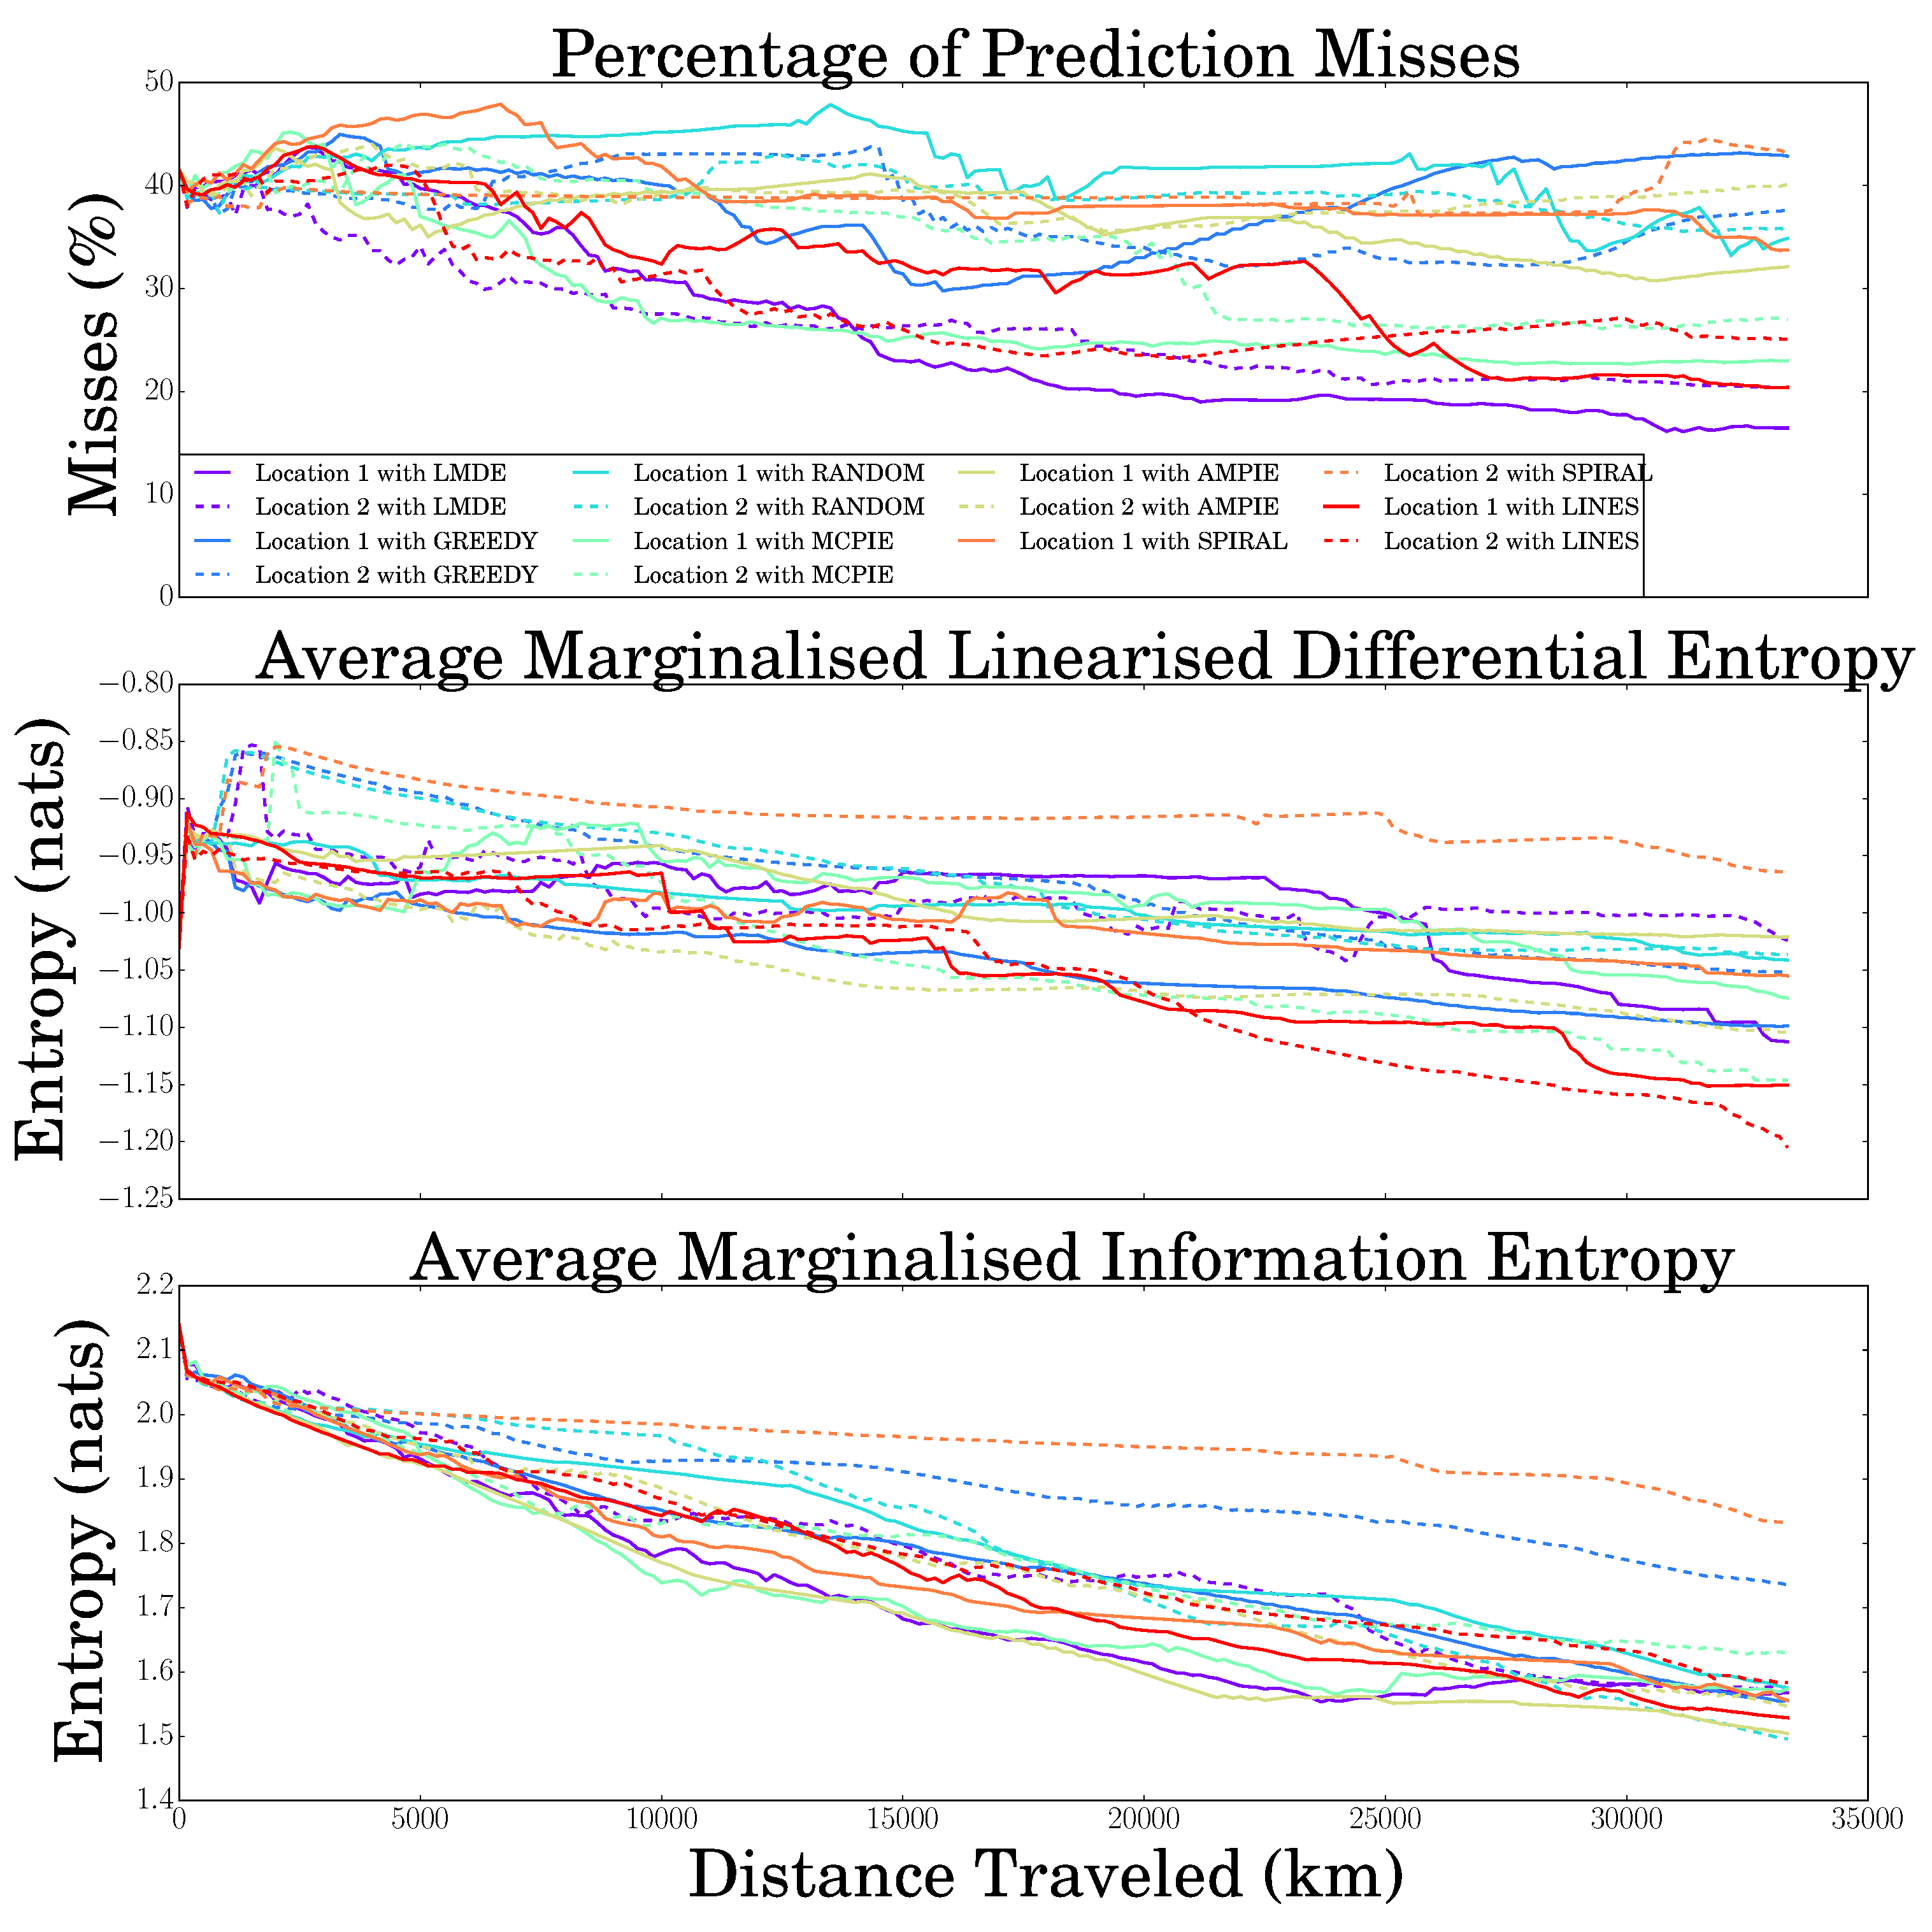
\includegraphics[width = \linewidth]{Figures/compare_methods.eps}
			\caption{Comparison of Informative Path Planning Methods}
			\label{Figure:CompareMethods}
			\end{figure}

			\begin{figure}[!htbp]
			\centering
				\includegraphics[width = \linewidth]{Figures/compare_locations.eps}
			\caption{Comparison of Initial Starting Positions}
			\label{Figure:CompareLocations}
			\end{figure}
				
			\begin{figure}[!htbp]
			\centering
				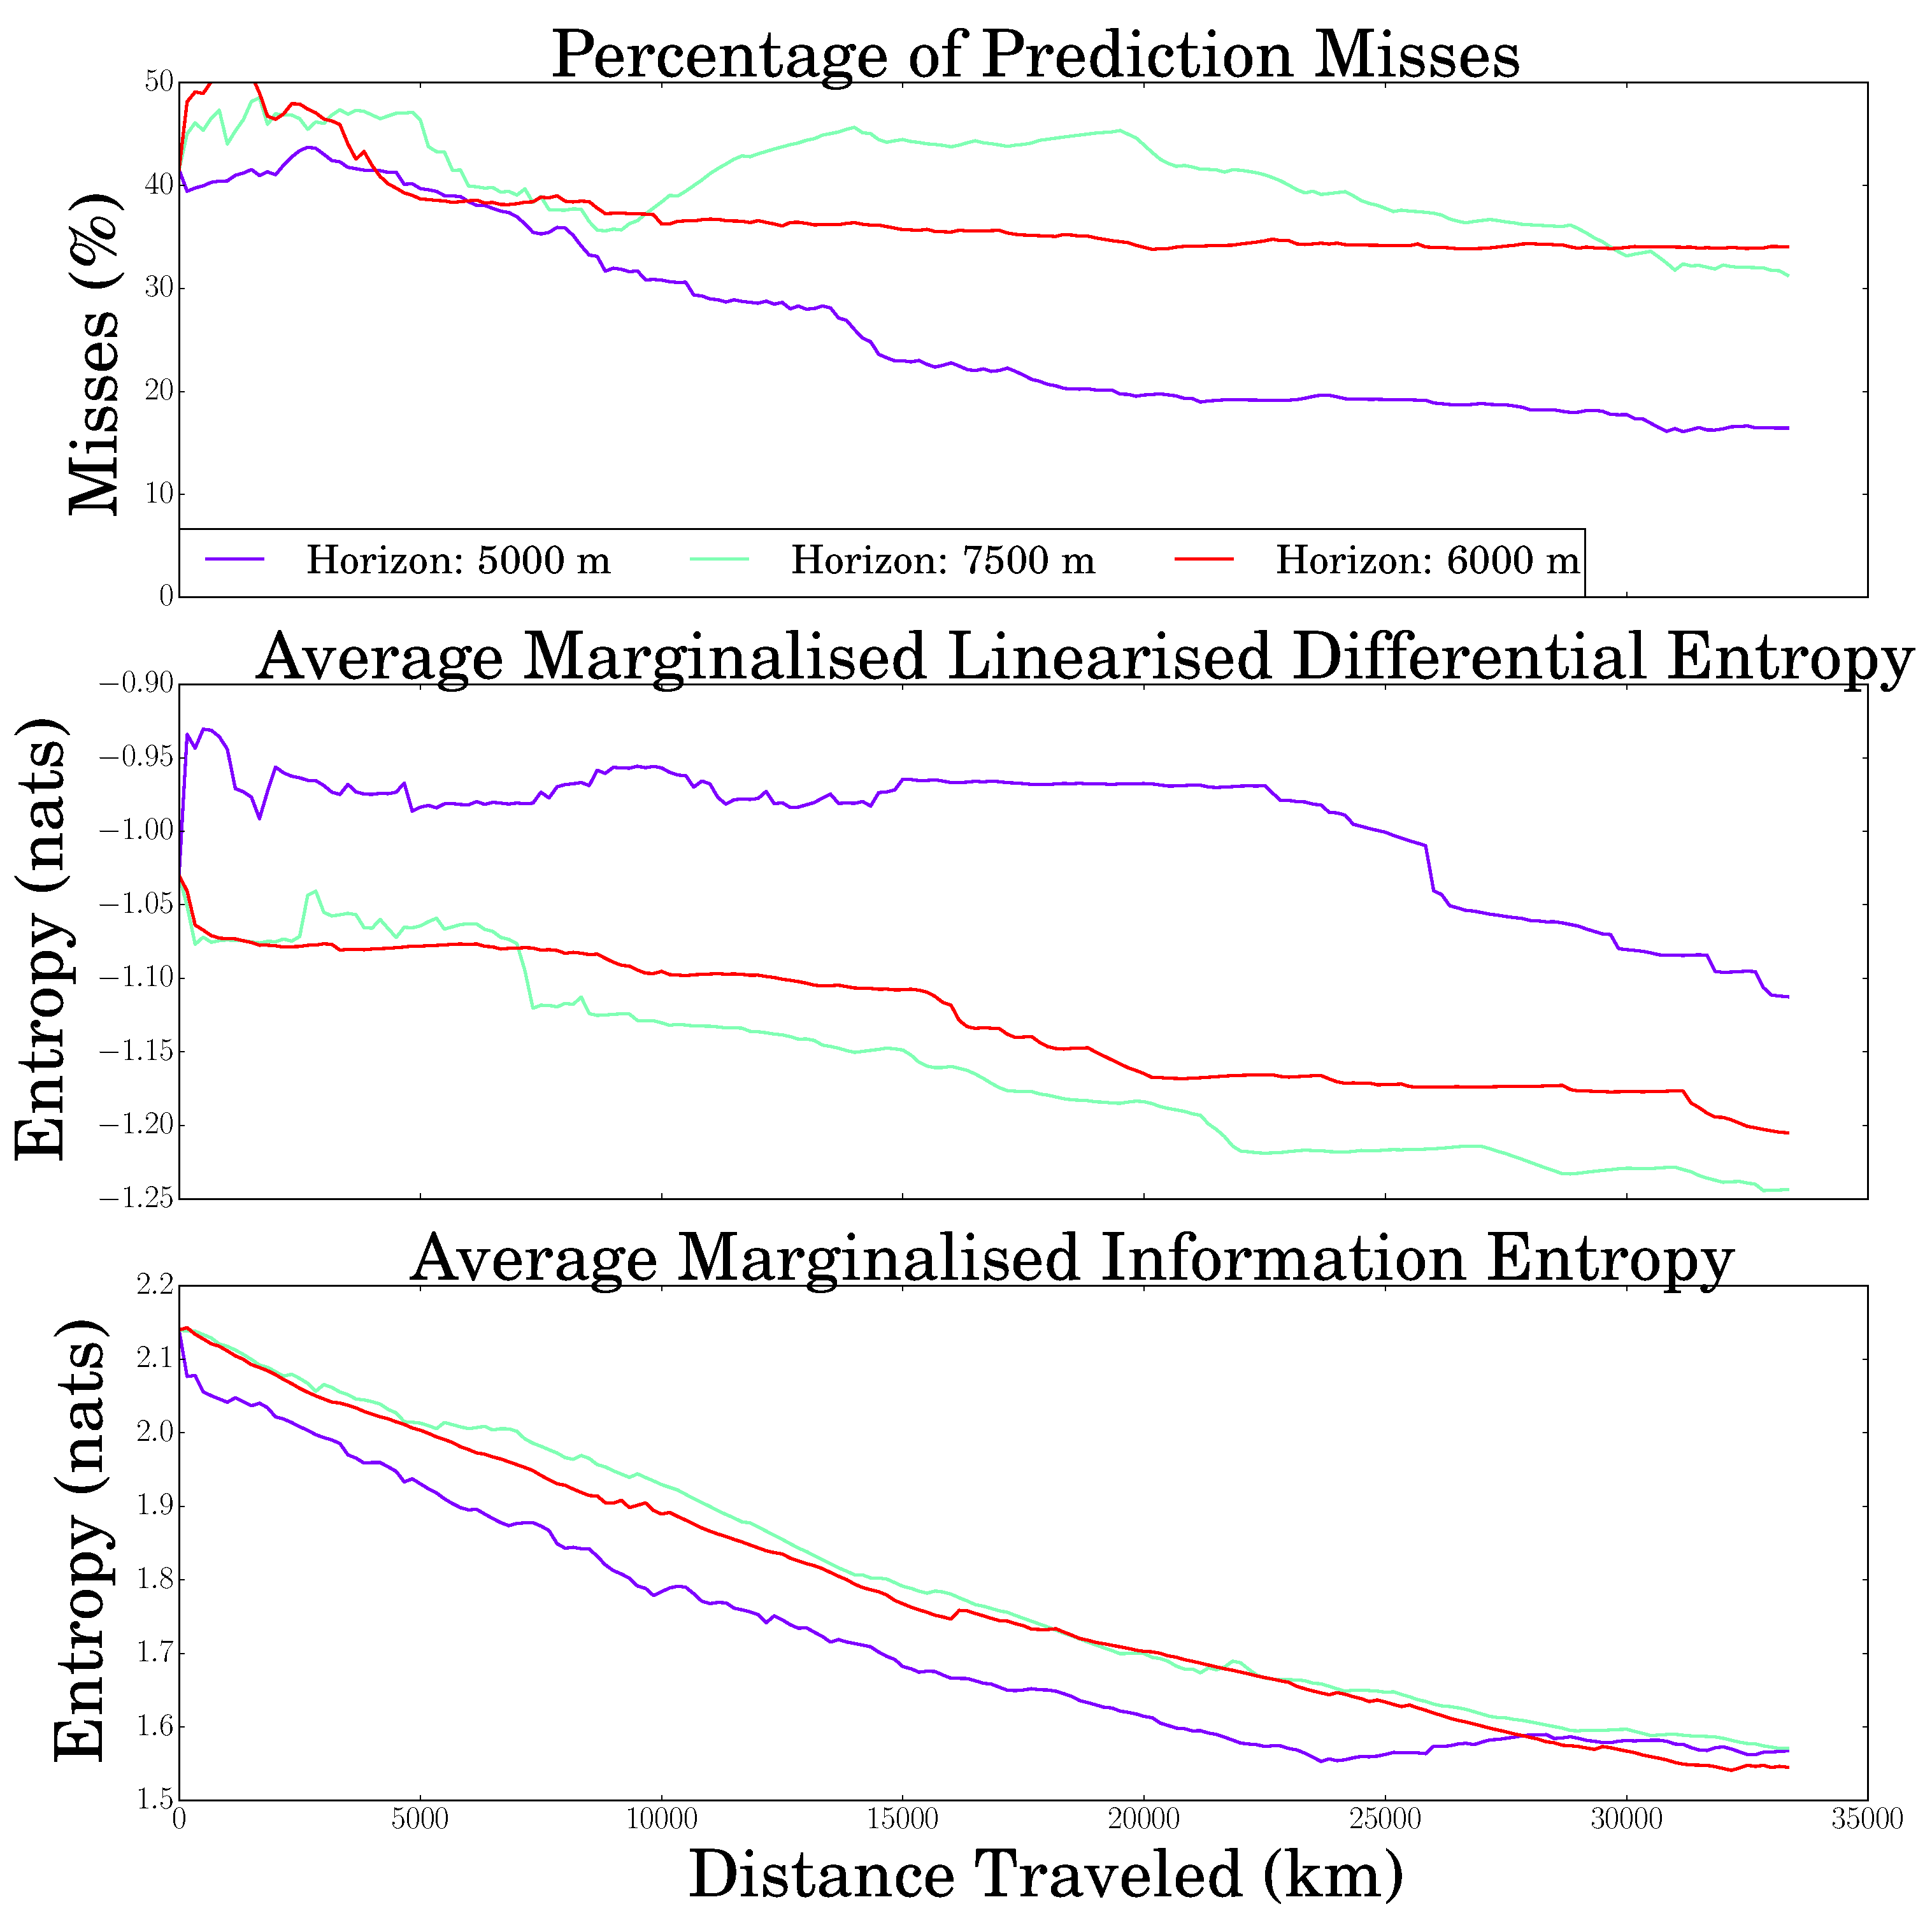
\includegraphics[width = \linewidth]{Figures/compare_horizons.eps}
			\caption{Comparison of Receding Horizon Lengths}
			\label{Figure:CompareHorizons}
			\end{figure}
				
								
	\section{Summary}

\chapter{Conclusion}
\lhead{Conclusion}
\label{Conclusion}

	This thesis investigates and develops informative seafloor exploration methods for benthic habitat mapping. Through concluding the work in informative path planning using linearised model differential entropy acquisition under receding horizon formulation, this section discusses the future outlook of this thesis work.
	
	\section{Contributions and Significance}
		
		Of the contributions listed in Section \ref{Introduction:Contribution}, the development and implementation of a new acquisition criterion, the linearised model differential entropy, and an informative path planning framework, the receding horizon formulation, are two of the most vital contributions of this thesis. Together, they form a complete informative path planning technique for benthic habitat mapping which is stable and relatively efficient compared to other methods. In effect, it allows a non-myopic, mutual informative exploration scheme that outperforms both Monte Carlo methods and other approaches without such properties. With a novel, principled, and tractable informative exploration policy that outperforms existing solutions, this concludes the mission of this thesis.
		
		Another major significance and implication of this work is its feasibility, tractability, and flexibility. Through developing a simple, efficient, and parallelisable multiclass classifier in the OVA and AVA scheme, coupled by improved probability fusion techniques, such a GP classification framework can be readily incorporated to other applications or extended further in the seafloor mapping domain.
		
%		Firstly, it avoids the need to compute acquisition criterion throughout the seafloor region, which is extremely costly in time for non-mutual information measures such as AMPIE, and furthurmore memory intensive for mutual information measures such as MCPIE and LMDE. As a result, this formulation make feasible the use of mutual information measures. Secondly, it allows a feedback structure to path planning and avoids executing outdated path plans. Thirdly, with an appropriate horizon structure, the method provides a balance between non-myopic planning and immediate feasibility.
		
%		Finally, these acquisition criteria and informative path planning schemes are evaluated in performance with the Scott Reef dataset, which reveals the effectiveness of MCPIE and especially LMDE acquisition approaches over non-mutual, myopic, and non-informative methods (Section \ref{InformativeSeafloorExploration:ScottReef}). 
	
	\section{Future Work and Implications}
	
		The work presented in this thesis calls for further work in improving the proposed informative path planning techniques and considering its implications.
		
		One of the most intriguing concept derived from this thesis is the relationship between prediction information entropy and model differential entropy. Semantic interpretations of their meanings have suggested that they are correspondingly similar to variance and bias, which are two sides of the ``coin'' of uncertainty. Further statistical analysis and investigation with probability theory could be interesting in revealing how these measures can be combined for a mutual information measure that allows the agent to intelligently discern uncertainty by variance and uncertainty by bias. With a hopeful outlook such a measure may be able to enable better acquisition properties for mapping problems that requires classification.
		
		On top of more investigations in the acquisition criteria, the path planning scheme itself can also be improved. The work of this thesis follows the common philosophy of transcribing a path planning problem in the continuous domain to the discrete domain. While this is a common and perfectly valid approach, it is certainty superseded by techniques that allow planning directly in the original continuous domain, in order to avoid discretisation approximations and hence limitations. 
		
		Nevertheless, there are also immediate work that can be investigated which builds on the current discretised formulation. Firstly, the horizon length could be reduced as the agent reaches the end of each mission. As no missions will continue indefinitely, it may be beneficial to let the agent know that its mission will terminate shortly such that it will switch to a more greedy approach before its time is up. More importantly, however, are the choices of the mission length and stopping criteria. Currently, the missions lengths are chosen based on experiences with past missions and the power limitations of the AUV. Nevertheless, it can be interesting to investigate the case where the AUV itself decides when to stop a mission, surface to sea level, and have a ship deliver it to a new location where it finds the most informative. This is based on the fact that underwater velocities are much slower than surface velocities. Such a scheme would involve the AUV constantly evaluating its surroundings against faraway regions for potential information. With appropriately devised loss functions, the AUV would decide whether it has explored the current area enough such that it is time to move to a new area.
			
		The tractability and accuracy of the methods developed above can also be improved. In terms of tractability, one of the major limitations of this work is that the datasets are large in quantity. Much work has been done in the machine learning community for efficient approximations of Gaussian process inference, such as sparse Gaussian process approximations where weak kernel covariances are discarded to save both memory and computational time. In terms of accuracy, while Laplace approximation achieves good performance, there are other approximation techniques that produce even more accurate results, although unfortunately at the expense of higher time complexity. Examples of such approximation methods are Expectation Propagation and Variance Inference \citep{GaussianProcessForMachineLearning}. The advantage of the work contributed in this thesis is that it is compatible with all such improvement techniques described in the literature.
		
		The work presented in this thesis is in fact not limited to the underwater domain. It can be used in any setting which requires building a map of discretely labeled objects. Typical examples include mapping the object occupancy of an area, aerial monitoring of agricultural lands with unmanned aerial vehicles, and terrain feature recognition with planetary exploration rovers. As such, the methods presented in this thesis could be tested on these scenarios to better evaluate performance, and further serve to inspire ways of improvements.
		
		The above application domains also motivate the need for a spatial-temporal model. In benthic habitat mapping, it is assumed that the true habitat map stay constant throughout the mapping procedure, so that observations made a long time ago are equally as valid as observations made recently. However, environmental monitoring problems such as object occupancy mapping of an dynamic environment involve a dynamically changing ground truth. While spatial-temporal models based on Gaussian processes have been investigated before \citep{Roman:SequentialBayesianOptimisation}, these methods typically only address the mapping of continuous targets which are regression problems. Further work building upon the Gaussian process classification scheme developed here is thus an interesting area to explore.
		
		Nevertheless, this thesis has presented a computationally viable approach to informative path planning through a novel acquisition function, the linearised model differential entropy. Under a receding horizon formulation, linearised model differential entropy acquisition has demonstrated significant improvement from traditional methods in the case of Scott Reef, which concludes the mission of this thesis.

	

%% ----------------------------------------------------------------
% Now begin the Appendices, including them as separate files

\addtocontents{toc}{\vspace{2em}} % Add a gap in the Contents, for aesthetics

\appendix % Cue to tell LaTeX that the following 'chapters' are Appendices

\chapter{Computational Aspects of Gaussian Processes}
\lhead{Computational Aspects of Gaussian Processes}
\label{Appendix:ComputationalAspects}

	\section{Numerical Stability}
	
		\subsection{Cholesky Decomposition}
		
		\subsection{Solving Triangular Matrix Equations}
		
		\subsection{Cholesky Jittering}
	
	\section{Time Complexity}
	\label{Appendix:ComputationalAspects:TimeComplexity}
	
		Reducing computational time
		
		\subsection{Numpy and Vectorisation}
		
		\subsection{Cholesky Update and Downdate}
		\label{Appendix:ComputationalAspects:TimeComplexity:CholeskyUpdateDowndate}
		
		\subsection{Caching learned GPs for fast prediction}
		
		\subsection{Parallelisation of GP learning and hyper-parameter batching}
		
		\subsection{Parallelisation of GP prediction and relevant subtleties}
		
		\subsection{Fast vectorised GP drawing for regression and classification}
		
	\section{Spatial Complexity}
	
		 Reducing memory requirements
		 
		\subsection{Symmetry of AVA multiclass classifier}
		
		\subsection{Creating predictor objects to modularise prediction}
		
	\section{Time \& Spatial Complexity}
	\label{Appendix:ComputationalAspects:TimeSpaceComplexity}
	
		\subsection{Avoiding full covariance computations}
		\label{Appendix:ComputationalAspects:TimeSpaceComplexity:CovarianceAvoidance}
		
		\subsection{Taking advantage of diagonal log-likelihood Hessians}
		\label{Appendix:ComputationalAspects:TimeSpaceComplexity:DiagonalHessians}
		
		 % Computational Aspects of Gaussian Processes
\chapter{Other Approximations for Gaussian Process Classification}
\lhead{Other Approximations for Gaussian Process Classification}
\label{Appendix:OtherApproximationsGaussianProcessClassification}

	\section{Expectation Propagation}
	
	\section{Variational Inference}
		 % Other Approximations for Gaussian Process Classification

%\input{Appendices/AppendixC} % Appendix Title

\addtocontents{toc}{\vspace{2em}}  % Add a gap in the Contents, for aesthetics
\backmatter

%% ----------------------------------------------------------------
\label{Bibliography}
\lhead{\emph{Bibliography}}  % Change the left side page header to "Bibliography"
\small
\bibliography{Bibliography}  % The references (bibliography) information are stored in the file named "Bibliography.bib"

\end{document}  % The End
%% ----------------------------------------------------------------